\documentclass[11pt]{article}
\usepackage[a4paper,margin=23mm]{geometry}
\usepackage{amsmath,amssymb,amsthm,mathtools}
\usepackage{tikz}
\numberwithin{equation}{section}
\usetikzlibrary{arrows.meta,patterns}
\usepackage[hyphens]{url}
\usepackage[pdfusetitle,colorlinks=true,linkcolor=blue,citecolor=blue,urlcolor=blue]{hyperref}
\newtheorem{theorem}{Theorem}[section]
\newtheorem{lemma}[theorem]{Lemma}
\newtheorem{proposition}[theorem]{Proposition}
\newtheorem{remark}[theorem]{Remark}
\newcommand{\Z}{\mathbb Z}
\newcommand{\Q}{\mathbb Q}
\newcommand{\C}{\mathbb C}
\newcommand{\T}{\mathcal T}
\newcommand{\D}{\mathcal D}
\newcommand{\Hh}{\mathcal H}
\newcommand{\tr}{\operatorname{tr}}
\newcommand{\pr}{\operatorname{pr}}

\title{Ambiently homeomorphic isolated hypersurface germs in \texorpdfstring{\(\C^4\)}{C4} with multiplicities four and five}
\author{OpenAI}
\date{September 27, 2026}
\begin{document}
\maketitle
\begin{abstract}
We give a negative answer to Zariski's multiplicity question in four
complex variables. We construct two reduced convergent holomorphic
function germs with isolated critical points and multiplicities four and
five whose zero-set germs are ambiently homeomorphic.
\end{abstract}
\section{Introduction}\label{sec:introduction}

Let \(f\in\mathbb C\{z_1,\ldots,z_N\}\) be a nonzero convergent
power series with \(f(0)=0\). The hypersurface germ \(V(f)\) is
\emph{reduced} when \(f\) has no repeated irreducible factor. Its
\emph{multiplicity} is
\(\operatorname{ord}_0f\), the least total degree of a nonzero term
of \(f\). Two hypersurface germs are \emph{ambiently homeomorphic}
if a homeomorphism between neighborhoods of the origin, fixing the
origin, takes one zero set onto the other. Equivalently, their ambient
pair germs \((\mathbb C^N,V(f),0)\) are homeomorphic.

Zariski's multiplicity question asks whether this embedded
topological germ determines multiplicity. He posed the question
explicitly in 1971 \cite{Zariski1971}, following his work on the
topology and equisingularity of plane curves
\cite{Zariski1932,Zariski1965}. In that classical setting, the
embedded topology determines the characteristic data of the branches
and their mutual intersection numbers, and hence the multiplicity;
see also the proof of \cite[Theorem~3.1]{KoikeParusinski2010}.
The higher-dimensional question asks whether this relation between
an equation's lowest degree and its embedded topology persists.

For an isolated critical point, Milnor's fibration gives a way to
study that topology through the \emph{link}
\(V(f)\cap S^{2N-1}_\varepsilon\) on a sufficiently small sphere
and the associated open book, whose complement fibration is
\(f/|f|\) \cite{Milnor1968}.
We answer Zariski's question negatively in four complex variables.

\begin{theorem}\label{thm:main}
There are reduced convergent holomorphic function germs
\(f_4,f_5\colon(\mathbb C^4,0)\to(\mathbb C,0)\), each with an isolated
critical point at the origin, such that
\[
   \operatorname{ord}_0f_4=4,\qquad
   \operatorname{ord}_0f_5=5,
\]
and a homeomorphism germ of ambient pairs
\[
   (\mathbb C^4,V(f_4),0)
      \;\cong\;
   (\mathbb C^4,V(f_5),0).
\]
\end{theorem}

The Milnor open book has a compact page whose middle-dimensional
cycles carry an integral Seifert form: it records the linking of a
cycle on a reference page with a cycle transported to a positive
neighboring page. For the open books on \(S^7\) used here, a
classification theorem turns a congruence of these integral forms
into an equivalence of the embedded links. The proof is therefore
organized around obtaining that integral congruence while retaining
the different orders of the equations.

\subsection*{Context and predecessors}

A major line of work concerns multiplicity within a deformation.
The Milnor number \(\mu\) is the dimension of the local algebra
defined by the first derivatives; for a convergent isolated germ it
is also the rank of the middle homology of the Milnor page.
Greuel and O'Shea independently proved equimultiplicity for
\(\mu\)-constant deformations of an isolated quasihomogeneous
singularity \cite{Greuel1986,OShea1987}.
Fernández de Bobadilla and Pełka proved the general family theorem:
every coefficientwise continuous path of formal power series with
finite constant Milnor number has constant multiplicity
\cite[Theorem~1.1]{BobadillaPelka2024}. The germs of
Theorem~\ref{thm:main} therefore cannot be endpoints of such a path.

The distinction between a family and an arbitrary pair is substantial.
Fernández de Bobadilla and Pełka's Example~8.6 gives a four-variable comparison:
double suspension of Du Bois--Michel plane curves with isometric
integral Seifert forms yields topologically equivalent germs of
equal multiplicity two, with no connecting \(\mu\)-constant family
\cite[Example~8.6]{BobadillaPelka2024}. Du Bois and Michel's plane
curves have different embedded types despite their isometric forms
\cite{DuBoisMichel1994}.

Another positive result retains geometric information beyond the
smooth embedded link. McLean proved that two isolated polynomial
singularities with embedded contactomorphic links have equal
multiplicity \cite[Theorem~1.1]{McLean2019}: the ambient sphere
map must preserve the natural contact structures as well as the
links. His Floer-theoretic characterization of multiplicity is a
starting point for the family theorem of Fernández de Bobadilla
and Pełka. The comparison in this paper uses smooth open books and
their integral Seifert forms.

Koike and Parusiński proposed high-power suspension of plane curves
with isometric Seifert forms as a route to topologically equivalent
four-variable germs, asking whether their Fukui numerical sets---the
sets of orders attained along analytic arcs---could differ. Their test of the Du Bois--Michel family gives
equal sets \cite[Section~5, pp.~294--296]{KoikeParusinski2010}. The
smooth sum and tensor calculation underlying our construction belongs
to the product theory of Sakamoto and Kauffman--Neumann
\cite{Sakamoto1974,KauffmanNeumann1977}.

A separate article by OpenAI, \emph{Ambiently homeomorphic isolated
hypersurfaces of multiplicities two and three}, constructs
real-coefficient, positive-weight homogeneous polynomials in one
finite complex dimension \(N>3\), divisible by eight, with orders
two and three and homeomorphic ambient germs
\cite[Theorem~1.1]{OpenAI2026Multiplicity23}. That construction uses weighted
homogeneous sums and spherical-link classification. The present
four-variable construction uses convergent equations in analytic
charts, a finite-map lattice calculation, and the nonspherical
open-book theorem. The two arguments are independent, and their
dimension, equation format, and exact multiplicities are distinct.
The ambient three-variable case remains untreated by either result.

\subsection*{Proof strategy}

The construction starts from the plane curve
\[
 h(X,T)=T(X-T^2)(X-2T^2)
\]
and two degree-four finite maps \(\pi_0,\pi_1\) obtained by projecting
smooth graph surfaces to the \((X,T)\)-plane. Their pullbacks \(d_i=h\circ\pi_i\)
are six-branch plane curves of the same embedded type, so their
integral plane Seifert forms are isometric. Thus the plane curves
themselves already have the same topology, whereas Du Bois and Michel's
examples separate topology from the abstract Seifert form. Here the
distinction lies in the maps to a common base curve, whose branch-degree
patterns differ. We retain their induced homology maps separately from
the abstract plane-form isometry. Section~\ref{sec:plane-cover} proves
that isometry and the separate pushforward and transfer identities.

A small rescaling of each graph equation smooths the cone \(yz=w^4\).
On each resulting smooth fourfold we use the function
\(h+w(y^a+z^b)\), with one common choice of \(a,b\). In
Section~\ref{sec:ambient-germs}, that choice is fixed before use;
analytic elimination gives orders five and four, and the subsequent
arc argument proves isolation. To compute the Milnor pages, we cut
each into an inner smoothing region and an exterior inherited from
the cone. An exterior cycle closes with an inner plane cycle only
when their boundary residues agree modulo four. This condition
depends on the pushforward for the particular graph map and is not
determined by the abstract plane Seifert form.
Sections~\ref{sec:tube}--\ref{sec:filling-summands} establish the
condition by a signed Mayer--Vietoris cut and an oriented Bockstein
calculation, then compute the two filling pairings in one convention.
The quotient by the cone's cyclic degree-four cover and its signed
integral gluing are established in this tube calculation. The resulting
lattice and form belong to the actual local Milnor page, as required
for the link theorem.

Two boundary directions of the cone page then give different
splittings of this integral lattice. Their coprime indices make
the associated rational maps integral at complementary sets of
primes, including the dyadic prime. Section~\ref{sec:fourfold-arithmetic}
compares those maps on the relevant quadratic and Hermitian
eigenspaces, lifts their discrepancy to the spin and special
unitary groups, and checks the real and lattice-stabilizer hypotheses
for strong approximation
\cite{Platonov1969,Platonov1970}
\cite[Theorem~2.3]{Rapinchuk2014}. This produces one integral
Seifert-form congruence.

Finally, Kato's classification of simple spinnable structures on
\(S^7\) applies to these Milnor open books without requiring their
bindings to be homotopy spheres \cite[Theorem~B]{Kato1974}.
Kato credits Durfee's independent work \cite{Durfee1974};
Saeki explains the singularity-facing formulation
\cite[Definition~2.1 and pp.~698--699]{Saeki1999}. After the page and
orientation hypotheses are checked, the integral congruence gives
an equivalence of embedded links. The analytic ambient-pair cone theorem
\cite[Theorem~1.4]{Massey2015LeCycles} extends it to the ambient pair
germs; this is the analytic form of the conical construction used by
Milnor \cite[Section~2]{Milnor1968}.

\section{Plane curves and the finite maps}\label{sec:plane-cover}

We first construct two finite maps to a common plane.  Their pulled-back
curves will supply isometric integral Seifert forms and the monodromy
sectors needed later.  We also retain the homology maps induced by each
projection, because those maps determine the integral boundary condition
in the fourfold construction.

Set
\begin{align*}
 h(X,T)&=T(X-T^2)(X-2T^2),\\
 q_1(u,w)&=(u-w-w^8)(u-w-2w^8)(u-w^2),\\
 q_2(u,w)&=q_1(u,w)-u^2 .
\end{align*}
We use two graph maps to the \((X,T)\)-plane:
\begin{align*}
 \pi_0(u,w)&=\bigl(\varphi(u,w),u\bigr),
    &\varphi(u,w)&=u^2+q_1(u,w),\\
 \pi_1(x,w)&=\bigl(x,\psi(x,w)\bigr),
    &\psi(x,w)&=u(u-w^2)q_2(u,w),\quad u=x+w.
\end{align*}
Write \(d_i=h\circ\pi_i\). For \(g\in\{h,d_0,d_1\}\), let \(F_g\)
denote the chosen sufficiently small compact oriented Milnor page of
\(g\). Set \(\mathcal H=F_h\), \(\mathcal D_i=F_{d_i}\), and put
\(H=H_1(\mathcal H;\mathbb Z)\), \(D_i=H_1(\mathcal D_i;\mathbb Z)\).
Throughout, \(s(a,b)\) is the ordered intersection of a filling of
\(a\) on a reference page with a filling of the positive neighboring-page
transport of \(b\), in the acyclic total Milnor tube.

\begin{lemma}[Plane data]\label{lem:plane-data}
Each \(\pi_i\) is a finite map germ of degree four. The curves \(d_i=0\)
are reduced, have isolated singularities at the origin, and have the same
six-branch embedded type. Their integral Milnor Seifert forms are
isometric, and each has Milnor number \(51\).
Let \(\Phi_5(t)=t^4+t^3+t^2+t+1\).  If \(M_h\) is the monodromy on
\(H_{\mathbb Q}=H\otimes\mathbb Q\), then
\[
 \dim_{\mathbb Q}\ker(M_h-I)=2,\qquad
 \dim_{\mathbb Q}\ker\Phi_5(M_h)=4.
\]
The monodromy on either \(D_i\otimes\mathbb C\) is semisimple at
eigenvalue \(1\) and at every primitive fifth root of unity.
\end{lemma}

\begin{proof}
\noindent\emph{Finite maps and branch contacts.}
At \(u=0\),
\[
 \varphi(0,w)=-w^4(1+w^7)(1+2w^7),
\]
and at \(x=0\),
\[
 \psi(0,w)=-w^4(1-w)+O(w^{19}).
\]
Weierstrass preparation in \(w\) therefore makes both graph projections
finite of degree four.

In the first graph \(d_0=u q_1q_2\). Introduce invertible local
coordinates \(x=u-w,\ t=u\). Two branches of \(q_1=0\) satisfy
\[
 x=A_e(t)=e\,t^8+O(t^{15}),\qquad e=1,2.
\]
The branch \(u=w^2\) satisfies \(t=x^2+O(x^3)\), and \(u=0\) gives \(t=0\).
The other two local branches arise from \(q_2=0\). Substituting \(u=vw^2\)
gives
\[
 q_2(vw^2,w)=w^4(v-1-v^2)+O(w^5).
\]
The two roots of \(v^2-v+1=0\) are simple; hence the implicit-function
theorem gives two branches
\[
 t=B_f(x)=f\,x^2+O(x^3),\qquad
 f=\frac{1+i\sqrt3}{2},\ \frac{1-i\sqrt3}{2}.
\]
These exhaust the local branches of \(q_2=0\): indeed
\(q_2(u,0)=u^2(u-1)\), so Weierstrass preparation in \(u\) has degree two.
Together with \(f=0,1\), these are four branches \(t=B_f(x)\).
All six are smooth and distinct.

In the second graph,
\[
 d_1=\psi(x,w)\bigl(x-\psi(x,w)^2\bigr)
                    \bigl(x-2\psi(x,w)^2\bigr).
\]
The four branches of \(\psi=0\) are exactly the four \(t=B_f(x)\)
above. Since \(\psi(0,w)=-w^4+O(w^5)\), the last two factors each have
a unique smooth branch \(x=e w^8+O(w^9)\), \(e=1,2\), and these read
\(x=e t^8+\text{higher terms}\) in \(t=x+w\). Thus both \(d_i\) are units
times products of two \(x=A_e(t)\) factors and four \(t=B_f(x)\) factors
with the same first distinguishing coefficients.

The two \(A\)-branches meet with multiplicity \(8\); any pair of
\(B\)-branches meets with multiplicity \(2\); a branch from each group
meets transversely. Hence
\[
 \delta(d_i)=8+\binom42\,2+2\cdot4=28,\qquad
 \mu(d_i)=2\delta(d_i)-6+1=51.
\]
\smallskip
\noindent\emph{The integral plane-form comparison.}
Interpolate only the terms above the displayed leading coefficients
and interpolate the nonvanishing units through units. This joins both
germs to the same leading product
\[
 d_\circ=(x-t^8)(x-2t^8)
       \prod_{f\in\{0,1,(1+i\sqrt3)/2,(1-i\sqrt3)/2\}}(t-fx^2).
\]
We now verify uniform isolation and boundary transversality along the
interpolation, which yield an oriented isotopy of its Milnor tubes.
In the sector \(|x|\le 2|t|\), if \(x/t^8\) stays bounded, weighted
rescaling has the noncritical model
\(t^4(x-t^8)(x-2t^8)\) at \(t=1\); its factors have distinct simple
roots, and its weighted Euler derivative excludes other critical
points. If \(|x/t^8|\to\infty\), all \(t-B_f(x)\) factors are
\(t(1+o(1))\), both \(x-A_e(t)\) factors are \(x(1+o(1))\), and
\(x\,\partial_x d/d\to2\). In the sector \(|t|\le2|x|\), the analogous
rescaling for bounded \(t/x^2\) gives
\(x^2\prod_f(t-fx^2)\); for \(|t/x^2|\to\infty\) one has
\(t\,\partial_t d/d\to4\). These estimates and their first
derivatives are uniform in the interpolation parameter after the
ball is shrunk. The six branch parametrizations also meet small
spheres transversely and remain disjoint there. The associated
Milnor tubes and boundary open books consequently form an oriented
isotopy. Transporting cycles and filling chains through it preserves
the integral Seifert pairing. Thus \(D_0\) and \(D_1\) have isometric
integral Seifert forms.

\smallskip
\noindent\emph{The required monodromy sectors.}
The plane-form comparison is now established. We finish by computing
the two sectors used in the arithmetic argument and excluding Jordan
blocks there. The three smooth branches of \(h\) have pairwise intersections
\(1,1,2\); thus \(\mu(h)=6\). The weighted rotation
\((X,T)\mapsto(\zeta^2X,\zeta T)\), \(\zeta^5=1\), preserves \(h\)
and has order five. Its nontrivial generator has no fixed point on
\(F_h\). Lefschetz therefore gives trace \(1\) on \(H_{\mathbb Q}\). Over
\(\mathbb Q\), a representation of the cyclic group of order five
is a sum of trivial and four-dimensional cyclotomic representations.
Its rank and trace equations force ranks \(2\) and \(4\), respectively.

It remains to justify the asserted Jordan condition for \(d_\circ\).
On a sufficiently small sphere, write its argument in the sector
\(|x|\le2|t|\) as the argument of
\[
 t^4(x-t^8)(x-2t^8)
 \prod_f(1-fx^2/t),
\]
and in \(|t|\le2|x|\) as the argument of
\[
 x^2\prod_f(t-fx^2)
 \prod_{e=1,2}(1-et^8/x).
\]
The displayed correction products are uniformly close to \(1\)
where used. Smooth cutoffs in the ratio \(|x|/|t|\) remove their
small arguments by an isotopy of argument fibrations. To see
regularity through that isotopy, use the angular fields of the
weighted rotations with rates \((8,1)/20\) on the \(t\)-side and
\((1,2)/10\) on the \(x\)-side. Each differentiates its corresponding
leading phase at rate one. On their common sector, both differentiate
\(2\arg x+4\arg t\) at rate one; the derivatives of the small
correction terms can be made arbitrarily small. Their convex angular
interpolation therefore remains positively transverse to every
intermediate phase. Near the binding only the appropriate weighted
field is used and is tangent to the binding. Thus the isotopy
preserves the open-book monodromy.

This periodic-piece description follows the plane-link calculus of \cite[Sections~11 and~13]{EisenbudNeumann1985}. The final phase in the overlap is \(2\theta_x+4\theta_t\).
Each regular phase level there has two annuli, both parametrized
by the radial ratio and the free angle \(\theta_t\), with the same
orientation. A single phase circuit exchanges their cores
\(\gamma_1,\gamma_2\) while preserving their angular orientations.
Outside the overlap, twenty circuits of either weighted rotation
return identically. Across each overlap annulus the
\(\theta_t\)-return varies from one turn on the \(t\)-side to four
turns on the \(x\)-side; hence the twentieth return makes the same
signed threefold Dehn twist on both annuli. The oriented boundary
of the \(t\)-side subsurface is \(\gamma_1+\gamma_2\) modulo actual
page-boundary circles. The latter lie in the radical of the surface
intersection form. Write \(M_\circ\) for the monodromy of
\(d_\circ\). Then
\[
 \operatorname{im}(M_\circ^{20}-I)\subseteq
 \mathbb Q(\gamma_1-\gamma_2),\qquad
 M_\circ(\gamma_1-\gamma_2)=-(\gamma_1-\gamma_2).
\]
Since \(M_\circ^{20}-I\) commutes with \(M_\circ\), it vanishes on the generalized
eigenspaces at \(1\) and at primitive fifth roots. The polynomial
\(z^{20}-1\) has simple roots; \(M_\circ\) is therefore semisimple on
those sectors.
\end{proof}

The two projections retain different degree profiles on the branches.
Here each tuple lists the degrees of the branches above the indicated
component of \(h=0\):
\[
\begin{array}{c|c|c}
\text{base branch} & \pi_0 & \pi_1\\ \hline
T=0     &(4)&(1,1,1,1)\\
X=T^2   &(1,1,2)&(4)\\
X=2T^2  &(2,2)&(4)
\end{array}
\]
We use the integral isometry of \(D_0\) and \(D_1\) only as an isometry
of their abstract forms; no compatibility with the two projections to
\(H\) is assumed.  The next lemma records the two maps on homology
associated with each projection.

\begin{lemma}[Finite-cover adjunction]\label{lem:cover-adjunction}
For \(i=0,1\), the page maps induce
\(\pi_{i*}:D_i\to H\) and a full-preimage transfer
\(\pi_i^!:H\to D_i\) satisfying
\[
 \pi_{i*}\pi_i^!=4\,\mathrm{id}_H .
\]
If \(s_h,s_{d_i}\) are the Seifert forms computed by ordered
filling-chain intersection in the total Milnor tubes, then
\[
 s_{d_i}(\pi_i^!a,b)=s_h(a,\pi_{i*}b),\qquad
 s_{d_i}(b,\pi_i^!a)=s_h(\pi_{i*}b,a).
\]
Consequently, after tensoring with \(\mathbb Q\),
\[
 D_{i,\mathbb Q}=(\ker\pi_{i*})_{\mathbb Q}
       \ \perp\ \pi_i^!H_{\mathbb Q},\qquad
 \operatorname{pr}_i(l)=l-\tfrac14\pi_i^!\pi_{i*}l
\]
is the projection onto \((\ker\pi_{i*})_{\mathbb Q}\) for both orders
of the form.
\end{lemma}

\begin{proof}
For an analytic germ \(f\) that is not locally constant, an ordinary
Milnor tube \(B_\epsilon\cap f^{-1}(D_\delta)\), with
\(0<\delta\ll\epsilon\ll1\), has contractible total; this is the
consequence of Milnor's proof recorded in
\cite[Theorem~1.8 and Remark~1.9]{Massey2015LeCycles}.
We compare the finite graph cuts used here with those ordinary tubes.
Choose finite proper graph representatives over one sufficiently small
closed base ball, and choose ordinary Milnor balls for \(h,d_i\) inside
the corresponding cuts. The branch parametrizations above allow regular
radii to be chosen so that the zero set in each closed intervening region
is exactly a disjoint union of branch annuli. The cut boundaries are
smooth near these annuli, and each annulus is transverse to both
boundaries. The function is a complex submersion normal to each annulus.
A field along the annulus directed from the inner boundary to the outer
one therefore extends, by this submersion, to a field tangent to the
nearby function levels. The disjoint flows give a value-preserving
collar of a neighborhood of the entire collection of annuli.
Properness makes the closed intervening region compact. Outside a
neighborhood of these annuli the absolute value of the function has a
positive lower bound, so a sufficiently small value disk confines the
intervening tube to that collar. Attaching the collar to the ordinary
tube preserves its homotopy type and gives regular lateral boundaries.
Thus these selected cut totals are acyclic. Choose nearby pages whose
base branch values lie in their interiors.
Represent a base class by loops avoiding these finitely many
values; the full preimage is a cycle upstairs.  This operation is
Poincar\'e--Lefschetz dual to pullback in relative first cohomology of
the pages, so it depends only on the homology class of the loops.
Counting the four sheets gives \(\pi_{i*}\pi_i^!=4\).

For the first pairing identity, fill the base loop \(a\) on the reference
page in the acyclic base total tube, and fill the positive neighboring-page
transport of \(b\) upstairs. Pull the first oriented surface chain back
through the finite holomorphic map, and push the second filling forward.
Put both fillings
and their boundary collars in general position. The base filling
meets the generic branch curve at isolated points, and the other
filling can be moved off their preimages; hence intersections relevant
to the pairing occur away from ramification. At each such intersection
the usual oriented projection formula counts the same local number
before and after pushforward. The finite map is over the value disk,
so it also commutes with positive nearby-page transport. This proves
the first identity; reversing the two filling arguments proves the
second. Finally, \(\pi_i^!H\) is rationally nondegenerate, since its
restricted form is \(4s_h\) by adjunction. Its two-sided orthogonal
complement is \(\ker\pi_{i*}\), and the displayed formula is the
corresponding projection.
\end{proof}

We have obtained the plane-form isometry together with a separate
pushforward, transfer, and rational projection for each graph.  The next
section uses the graph equations to construct the two smooth fourfold
germs and to read their ordinary orders in analytic coordinates.

\section{Smooth ambient germs and their ordinary orders}
\label{sec:ambient-germs}

Starting from the two graph maps, we now construct the smooth fourfold
germs and compute the first nonzero terms of their functions.  We first
fix one parameter choice for both graphs.  The same choice will satisfy
the later arithmetic requirements, while the estimates proved here
supply the local isolation argument in Lemma~\ref{lem:isolation}.

\begin{lemma}[One common parameter choice]\label{lem:simultaneous-parameters}
For every sufficiently large integer \(r\), choose an integer \(n_0\)
such that
\[
 n_0\equiv1\pmod{2^r},\qquad n_0\equiv2\pmod5,\qquad
 n_0>5\cdot2^r,
\]
and define
\begin{align*}
 n_1&=n_0+5\cdot2^r,&
 a&=(n_0^2-1)/4,& b&=(n_1^2-1)/4,\\
 \alpha&=\frac{4b}{a+b},&
 \beta&=\frac{4a}{a+b}.
\end{align*}
Then \(a,b\) are positive comparable integers,
\(n_0,n_1\equiv1\pmod4\), and \(\gcd(n_0,n_1)=1\).
Moreover
\[
 \alpha+\beta=4,\qquad a\alpha=b\beta,\qquad
 \frac{(a-2)\alpha}{4}>4,\qquad
 \frac{(b-2)\beta}{4}>4.
\]
\end{lemma}

\begin{proof}
The Chinese remainder theorem supplies arbitrarily large \(n_0\)
with the two congruences, so the strict lower bound can also be imposed.
For large \(r\) we have \(r\ge2\), and both \(n_j\) are \(1\pmod4\);
therefore \(a,b\) are integers.  The lower bound on \(n_0\) gives
\(n_0<n_1<2n_0\), so \(a,b\) are positive, comparable, and grow
without bound with \(r\).  A common divisor of \(n_0,n_1\) divides
\(5\cdot2^r\).  Both integers are odd and \(2\pmod5\), proving
\(\gcd(n_0,n_1)=1\).

The identities for \(\alpha,\beta\) follow from their definitions.
Since \(b>a\),
\[
 \frac{(a-2)\alpha}{4}
 =\frac{ab}{a+b}-\frac{2b}{a+b}
 >\frac a2-2,\qquad
 \frac{(b-2)\beta}{4}
 =\frac{ab}{a+b}-\frac{2a}{a+b}
 >\frac a2-2.
\]
The right sides exceed four for sufficiently large \(r\).
In particular, the chosen \(a,b\) exceed four.
\end{proof}

Fix this choice for the rest of the paper, and set
\[
 g=\gcd(a,b),\qquad m=4ab+a+b.
\]
Lemma~\ref{lem:parameter-indices} proves the additional arithmetic
properties of these same integers: \(a,b\equiv2\pmod5\),
\(5\nmid g\), \(g\ge2^{r-1}>5\), and, for each \(q\in\{1,4\}\),
the existence of positive integers \(i,j\) satisfying
\[
 i\equiv j\pmod4,\qquad \frac{bi+aj}{m}=\frac q5.
\]
The deformation parameter \(s\) will be chosen sufficiently small only
after this tuple has been fixed.

Put \(p=(X,T)\).  Let \(R_0(p,w)\) and \(R_1(p,w)\) be the monic
degree-four Weierstrass polynomials in the graph equations
\begin{align*}
 X-T^2-q_1(T,w)&=U_0(p,w)R_0(p,w),\\
 T-\psi(X,w)&=U_1(p,w)R_1(p,w),
\end{align*}
where \(U_0,U_1\) are analytic units.  For a fixed small real \(s>0\),
set
\begin{align*}
 R_{i,s}(p,w)&=s^4R_i(p,w/s),\\
 C_{i,s}&=\{(p,y,z,w):yz=R_{i,s}(p,w)\},\\
 f_{i,s}&=\left.h(p)+w(y^a+z^b)\right|_{C_{i,s}} .
\end{align*}

\begin{proposition}[Analytic germs and their orders]
\label{prop:ambient-orders}
For the parameters of Lemma~\ref{lem:simultaneous-parameters}
and every sufficiently small \(s>0\), each \(C_{i,s}\) is a smooth
complex fourfold near the origin, and \(f_{i,s}\) has an isolated
critical point there, as proved in Lemma~\ref{lem:isolation}. After solving the smooth ambient equations
in analytic local coordinates, \(f_{0,s}\) has order five and
\(f_{1,s}\) has order four. Both are reduced convergent germs.
\end{proposition}

\begin{proof}
The specializations in Lemma~\ref{lem:plane-data} give
\(R_i(0,w)=w^4\) and \(U_i(0)=1\).  Hence
\[
 \partial_XR_0(0)=1,\qquad \partial_TR_1(0)=1.
\]
These derivatives remain nonzero along the respective local
root loci after shrinking.  For \(s>0\), the corresponding derivatives
of \(R_{i,s}\) are multiplied by the nonzero factor \(s^4\).
At a point of \(C_{i,s}\) with
\(y\ne0\) or \(z\ne0\), its defining equation has a nonzero
vertical derivative; at \(y=z=0\), one of the displayed base
derivatives is nonzero. Thus the ambient germs are smooth.

The two ambient equations are equivalently the implicit equations
\begin{align*}
 X&=T^2+q_1(T,w/s)+s^{-4}U_0(p,w/s)yz,\\
 T&=\psi(X,w/s)+s^{-4}U_1(p,w/s)yz,
\end{align*}
respectively.  In the first, \(q_1(T,w/s)\) has ordinary order at least
three.  Since \(U_0(0)=1\), analytic implicit solution gives
\[
 X=T^2+s^{-4}yz+O_{\ge3}(T,y,z,w).
\]
In the second graph \(q_2=q_1-u^2\) has order two, and
\(\psi=u(u-w^2)q_2\) has order four. Therefore
\[
 T=s^{-4}yz+O_{\ge3}(X,y,z,w).
\]
Here \(s\) is fixed and \(O_{\ge j}\) denotes terms of ordinary
total degree at least \(j\); in particular all \(w^4\) terms
lie in these remainders. The chosen \(a,b\) exceed four, so
\(w(y^a+z^b)\) has order greater than five. Substitution in \(h\)
gives the nonzero initial forms
\[
 \operatorname{in}(f_{0,s})
   =T(s^{-4}yz)(s^{-4}yz-T^2),\qquad
 \operatorname{in}(f_{1,s})=s^{-4}yzX^2.
\]
They have degrees five and four, respectively.

It remains to justify the isolated critical points claimed in the
proposition.  The input from the base curve is the following explicit
gradient estimate.  Along an analytic arc, let \(\nu\) denote order in
the arc parameter, with \(\nu 0=\infty\); for a vector, \(\nu\) is the
minimum of its component orders.  If an analytic arc \(p=(X,T)\ne0\) has
\(m_0=\nu p=\min(\nu X,\nu T)\), then
\begin{equation}\label{eq:plane-gradient}
 \nu\nabla h\le4m_0.
\end{equation}
Indeed
\(h_X=T(2X-3T^2)\) and
\(h_T=X^2-9T^2X+10T^4\).
If \(\nu X<2\nu T\), the first term of \(h_T\) has order
\(2\nu X\le4m_0\). If \(\nu X>2\nu T\), the term
\(-3T^3\) of \(h_X\) has order \(3\nu T\le4m_0\).
In the equality case, put \(X/T^2=c+\text{higher terms}\);
\(2c-3\) and \(c^2-9c+10\) have no common root, so one
derivative has order at most \(4\nu T=4m_0\).
The cases in which one coordinate vanishes identically are
immediate.

The full multiplier argument, including the cases where a vertical
variable vanishes, is given in Lemma~\ref{lem:isolation}; it uses the
two strict bounds in Lemma~\ref{lem:simultaneous-parameters} with the
gradient exponent \(4\) just proved.

Finally, if a convergent hypersurface germ had a repeated
irreducible factor, its gradient would vanish at generic
nonzero smooth points of that factor. Lemma~\ref{lem:isolation} therefore also implies reducedness.
\end{proof}

Choose one \(s>0\) below the thresholds for both graphs and choose
analytic charts \(C_{i,s}\cong(\mathbb C^4,0)\).  The germs in
Theorem~\ref{thm:main} are then \(f_5=f_{0,s}\) and \(f_4=f_{1,s}\).

\section{The cone tube and integral gluing}\label{sec:tube}

We now compute the integral middle homology and ordered Seifert
pairing for the functions constructed in the preceding section.
The calculation keeps the projection and transfer of each graph
map visible: these maps determine how cycles close across the
boundary of the smoothing region. Throughout this calculation
\(k=4\); the letter \(k\) records the covering degree in the formulas.

Let \(p=(X,T)\), \(h=T(X-T^2)(X-2T^2)\), and let
\(\pi:(\C^2,0)\to(\C^2,0)\) be one of the two degree-four finite
graph maps \(\pi_i\), with \(i\in\{0,1\}\) in the construction. Write \(d=h\circ\pi\), and let
\[
 R(p,w)=w^k+\sum_{j<k}A_j(p)w^j,\qquad k=4,
\]
be its prepared equation, so \(A_j(0)=0\) and \(R(0,w)=w^k\).
The root surface \(R=0\) is smooth near the origin; one component of \(R_p\)
is a unit. For \(s>0\), put \(R_s(p,w)=s^kR(p,w/s)\) and
\[
C_s=\{(p,y,z,w):yz=R_s(p,w)\},\qquad
f_s=h(p)+P(y,z,w),\quad P=w(y^a+z^b).
\]
The germ \(C_s\) is smooth of complex dimension four. The tube
statement below is formulated for any sufficiently large positive
integers \(a,b\) satisfying its two displayed inequalities. For the
two germs of this paper we use the single tuple already fixed in
Lemma~\ref{lem:simultaneous-parameters}. For such a qualifying pair, set
\[
\alpha=\frac{kb}{a+b},\qquad \beta=\frac{ka}{a+b},\qquad
\alpha+\beta=k,\qquad a\alpha=b\beta.
\]
Let \(\Hh,\D\) be the pages of \(h,d\). Let \(Q\) be a small
fiber \(P^{-1}(c)\) in the cone \(\{yz=w^k\}\), with \(c\ne0\);
it lies entirely in the smooth nonvertex locus.
Their middle homology groups are
\(H=H_1(\Hh;\Z)\), \(D=H_1(\D;\Z)\), and \(E=H_1(Q;\Z)\).
The finite map has projection and transfer \(\pi_*:D\to H\),
\(\pi^!:H\to D\), with \(\pi_*\pi^!=k\). Put
\(K=\ker\pi_*\) and
\(\pr l=l-k^{-1}\pi^!\pi_*l\in K_\Q\).
The cone link \(L\) is a lens space, \(H_1(L)=\Z/k\), and
\(\tau:E\to\Z/k\) is induced by weighted radial projection
\(Q\to L\), equivalently by page inclusion in the link open-book model.
Write \(s_h,s_d\) for the tube filling forms in the ordered
neighboring-page convention fixed in Section~\ref{sec:plane-cover}.
The cyclic map \((U,V)\mapsto(U^k,V^k,UV)\) to the cone pulls
\(P\) back to \(\widetilde P(U,V)=UV(U^{ka}+V^{kb})\).
Let \(\widetilde Q\) be its plane Milnor page, and let
\(\widetilde s\) be its plane-page form. The cyclic cover of the
nonvertex cone gives a full-lift map
\(\tr:E\to H_1(\widetilde Q;\Z)\); define
\[
 e(v,v')=\frac1k\widetilde s(\tr v,\tr v').
\]
This form is a priori rational because of the factor \(1/k\).
The theorem below specifies the integral page lattice on which
the rational form is evaluated.

\begin{theorem}[Tube, lattice, and pairing]\label{thm:tube}
For sufficiently large \(a,b\) satisfying
\[
 \frac{(a-2)\alpha}{k}>L_0,\qquad
 \frac{(b-2)\beta}{k}>L_0,
\]
where \(L_0=4\) is the gradient exponent in
\eqref{eq:plane-gradient}, and for sufficiently small \(s>0\), the germ
\(f_s:C_s\to\C\) has its sole critical point at the origin in a fixed
small tube. Its integral Milnor lattice, in rational coordinates, is
\begin{equation}
\Lambda_\pi=
\left\{(\pr l,z): l\in D,\ z\in H\otimes E,\quad
\pi_*l\bmod kH=(1\otimes\tau)z\right\}
\subset K_\Q\oplus(H\otimes E)_\Q.
\label{eq:tube-1}
\end{equation}
The rational orthogonal filling form on these coordinates is
\begin{equation}
  -s_d|_K\ \perp\ (s_h\otimes e).
\label{eq:tube-2}
\end{equation}
The lattice and form are those of a genuine local Milnor page of
\(f_s\) in the smooth ambient germ \(C_s\).
\end{theorem}

In \eqref{eq:tube-1}, \(z\) records the exterior product class,
while \(l\) indexes an inner closing chain. The equality of residues
is the condition for these pieces to close, and \(\pr l\) is the
resulting rational inner coordinate.

Section~\ref{sec:boundary-geometry} supplies boundary regularity,
compatible continuations, and isolation.
Section~\ref{sec:circle-collapse} computes the inner homology and
proves acyclicity of the large total. It then compares the large and
local total/page pairs, identifying the page homology and ordered
form with the ordinary local Milnor data. Its signed exterior cut
determines which exterior cycles extend.
Section~\ref{sec:integral-lattice}
then determines the integral lattice in these rational coordinates through the
Bockstein and transfer, and Section~\ref{sec:filling-summands}
computes the two ordered filling forms.

\section{Boundary geometry and the Milnor representative}\label{sec:boundary-geometry}

The tube calculation must describe a genuine local Milnor page.
We choose a larger representative whose inner and exterior
parts admit the required continuations. This section proves its
boundary regularity, constructs compatible changes of model on the
inner and exterior pieces, and proves isolation. The next section
uses those models to prove acyclicity and then compares this
representative with an ordinary small Milnor tube.

Fix \(M>3\), with \(M^{a+b}>1+k\max(a,b)\), and for
\(t>0\) set
\[
Y_t=\{|y|\le Mt^\alpha,\ |z|\le Mt^\beta,\ |w|\le t\}.
\]
Choose a sufficiently small base ball \(\mathcal B\) for both
plane tubes. Then choose \(\rho>0\), \(\varepsilon>0\),
\(\delta>0\), \(\lambda>0\), and \(s>0\), in that order, with
\begin{equation}
0<\delta<\varepsilon/4,\qquad 0<\lambda\ll\rho,\qquad
\sup_{Y_\lambda}|P|<\delta/4,
\label{eq:tube-3}
\end{equation}
and with every root of \(R_s(p,\cdot)\), for \(p\in\mathcal B\),
in \(|w|<\lambda/4\). The last condition follows because the roots
are \(s\) times the roots of \(R(p,\cdot)\) on the compact base cut.
Our larger closed total tube is
\begin{equation}
\widehat\T_s=
\{p\in\mathcal B,\ |h|\le\varepsilon,\ (y,z,w)\in Y_\rho,\
yz=R_s(p,w),\ |h+P|\le\delta\},
\label{eq:tube-4}
\end{equation}
and \(\T_s=f_s^{-1}(c)\cap\widehat\T_s\) for \(|c|=\delta\).
Write \(X_s\) for the same cut set with the final inequality
\(|h+P|\le\delta\) omitted. Its outer lateral strata are formed by
the base-ball, \(|h|=\varepsilon\), and \(\partial Y_\rho\) faces
and their active corners.
Let \(W\) be the part of \(\T_s\) in \(Y_\lambda\), let
\(M_{\rm ext}\) be the part of \(\T_s\) outside the interior of
\(Y_\lambda\), and let \(J\) be their
bicollared interface. Hats denote the corresponding total disk pieces.
The auxiliary interface \(J\) is an interior cut of \(X_s\), rather
than one of its outer lateral strata.

\subsection{Regularity on the outer boundary}

\begin{lemma}[Outer boundary regularity]\label{lem:boundary}
For every sufficiently small fixed \(s>0\), the map \(f_s\) on
the compact outer lateral boundary of \(X_s\) over
\(\{|v|\le\delta\}\) is proper, and its restriction to every
stratum has real rank two throughout that disk.
In particular, all active lateral faces and corners of \eqref{eq:tube-4}
are independent of the horizontal face over \(|f_s|=\delta\).
The horizontal boundary map is proper on the union of lateral
strata and a submersion on each stratum.
\end{lemma}
\begin{proof}
We first estimate the vertical faces and corners, then prove
uniform regularity on the remaining outer strata.

At \(s=0\) the vertical equation is \(yz=w^k\). Its link on
\(\partial Y_t\) is the cyclic quotient of a 3-sphere, hence a lens
space. The cone is smooth away from its vertex. The \(y\)- and
\(z\)-faces cannot meet: if both were active, then
\(|yz|=M^2t^k>|w|^k\). On the \(y\)-face,
\begin{equation}
\left|\frac{z^b}{y^a}\right|
\le M^{-(a+b)}\left(\frac{|w|}{t}\right)^{kb}<1.
\label{eq:tube-5}
\end{equation}
After eliminating \(z=w^k/y\), the free derivative is
\(P_w=y^a+(kb+1)z^b\), which is nonzero by the stronger choice
of \(M\). The \(z\)-face is symmetric, with
\(P_w=z^b+(ka+1)y^a\). These estimates persist for small
positive \(s\) by uniform convergence of \(R_s\) and
\(\partial_wR_s\) on the fixed outer face.
At a \(y/w\) corner the bound
\begin{equation}
 |P|\ge t^{1+a\alpha}(M^a-M^{-b})>0
\label{eq:tube-6}
\end{equation}
holds; similarly at a \(z/w\) corner. Choose
\(\varepsilon+\delta\) below both lower bounds at \(t=\rho\).
On the \(w\)-face, near a zero of \(P\) with \(w\ne0\),
use \(y\) as the free coordinate and \(z=w^k/y\).
Then \(dP(\partial_{\log y})=w(ay^a-bz^b)
=w(a+b)y^a\ne0\) at \(P=0\).
On the compact outer \(w\)-face, this nonvanishing persists in
one uniform small-value neighborhood; choose
\(\varepsilon+\delta\) within it.
The quotient expression \(\widetilde P=UV(U^{ka}+V^{kb})\)
also shows submersivity of \(P\) in the nonvertex cone interior:
if \(U,V\ne0\), its two partials cannot vanish simultaneously
because that would imply \((ka+1)(kb+1)=1\);
on each axis the transverse partial is nonzero.
These calculations cover the vertical faces and corners near the
small values used in \eqref{eq:tube-4}.

To finish the regularity claim on the genuine outer strata, consider
a sequence approaching the cone vertex while \(s\to0\), and let
\(\varrho=\max(|y|^{1/\alpha},|z|^{1/\beta},|w|)\).
If \(\varrho/s\to\infty\), weighted rescaling by \(\varrho\) gives smooth
convergence at a nonvertex cone point; all lower Weierstrass terms
vanish because \(A_j\) is bounded and \((s/\varrho)^{k-j}\to0\).
If \(\varrho/s\) is bounded, rescale by \(s\), with
\((Y,Z,u)=(y/s^\alpha,z/s^\beta,w/s)\); the limit is the smooth
model \(YZ=R(p,u)\). For \((Y,Z)\ne(0,0)\)
the base projection is a submersion; at \(Y=Z=0\) its differential
contains the tangent image of the smooth root graph.
The specified \(h,d\) Milnor cuts have the needed transversality
on \(\partial\mathcal B\), including corners with \(|h|=\varepsilon\).
For the actual function \(f_s\), these arguments give the stated
outer lateral regularity over the whole value disk. Indeed
\(\lvert P\rvert\le\varepsilon+\delta\) whenever
\(\lvert f_s\rvert\le\delta\), so all the outer vertical-face
estimates apply throughout that disk, also at their intersections
with base faces because the free vertical directions keep the base
fixed. On an outer stratum with no vertical face, a hypothetical
failure with unbounded \(\varrho/s\) would contradict submersivity of
\(P\) on the nonvertex cone after rescaling. If \(\varrho/s\) is bounded,
then \(P=s^{1+a\alpha}u(Y^a+Z^b)=o(1)\) in the smooth rescaled
model. The face \(\lvert h\rvert=\varepsilon\) is then absent over
\(\lvert f_s\rvert\le\delta<\varepsilon/4\). On the remaining
base-ball face, the boundary fibrations of \(h\) and \(d\) over
their full small value disks give rank two, respectively where
\((Y,Z)\ne(0,0)\) and on the smooth root graph. Compactness and
the preceding smooth convergence preserve these ranks for small
\(s\). This assertion concerns the outer cuts of \(X_s\); it
does not assert disk-wide submersivity on the auxiliary \(J\).
The remaining interior critical-point possibility is excluded in
Lemma~\ref{lem:isolation}. All statements here are open in compact
families of smooth strata, so one uniform upper bound on \(s\)
works for all strata.

\end{proof}

\subsection{Compatible continuations and the lens circle}

The inner and exterior computations use different models. To glue
classes computed in them, we must carry the same oriented lens circle
over each labeled base loop. This retains the labeling of the
interface tori; in Section~\ref{sec:integral-lattice} it will identify
the full finite-map transfer.

For \(|c|=\delta\), write \(\Hh_c=\mathcal B\cap\{h=c\}\).
Choose a smooth \(h\)-trivialization of pairs, respecting the
base-ball boundary, \(\Phi(p_0,q)\), over a disk about \(c\)
containing \(\{|q-c|\le\delta/4\}\), with
\(p_0\in\Hh_c\), \(\Phi(p_0,c)=p_0\), and
\(h(\Phi(p_0,q))=q\). Set \(w_0=\lambda/2\).

\begin{lemma}[Compatible continuations]\label{lem:continuations}
For sufficiently small \(s>0\), the exterior total/page pairs continue
to \(s=0\). On the inner part, the sublevel totals and
horizontal-boundary fibrations continue from \(h+P\) to \(h\)
through \(h+\theta P\), \(0\le\theta\le1\). These continuations preserve the complex
value on the horizontal boundary and agree on \(J\) up to isotopy
through their two-parameter rectangle.

They can be chosen to preserve the label \(p_0\), the coordinate
\(w_0\), and the exact positive \(y\)-angle \(\phi\) on the
interface circles characterized by
\[
 p=\Phi(p_0,q),\qquad w=w_0,\qquad
 y=M\lambda^\alpha e^{i\phi},\qquad h(p)+\theta P(y,z,w)=c.
\]
Here \(z=R_s(p,w_0)/y\), and \(q\) is the unique value near \(c\)
that satisfies these equations. The inner continuation is an isotopy
of sublevel totals; value preservation is required on its horizontal
boundary, not through its critical region.
\end{lemma}
\begin{proof}
At the inner interface, \eqref{eq:tube-3} and \(|h+\theta P|=\delta\) imply
\begin{equation}
3\delta/4\le |h|\le5\delta/4<\varepsilon
\quad(0\le\theta\le1).
\label{eq:tube-7}
\end{equation}
Thus \(h\) is regular there, including on its base-ball cut, and
the \(|h|=\varepsilon\) cut is absent. On the inner \(w\)-face,
\eqref{eq:tube-7} makes \(h\) regular, and \(\lambda\) can be
decreased until \(P\) is small in \(C^1\) there.
The zero-parameter cone is
smooth along this interface, so the same assertion holds throughout
the \((s,\theta)\) rectangle for small \(s\). We use regularity
of the horizontal boundary to isotope the \emph{sublevel totals}
as manifolds with corners; we do not assert that \(h\) is submersive
through every value in the disk at \(\theta=0\).

We first construct the prescribed circle family. For fixed
\((p_0,\phi,\theta,s)\), solve
\[
q+\theta P\left(y,\frac{R_s(\Phi(p_0,q),w_0)}y,w_0\right)=c
\]
for \(q\) near \(c\), then set
\(p=\Phi(p_0,q)\) and \(z=R_s(p,w_0)/y\).
The root bound gives
\(\lvert R_s(p,w_0)\rvert\le(3\lambda/4)^k\), so these circles
lie on the \(y\)-face and strictly away from the \(z\)- and
\(w\)-faces. Thus the small bound for \(P\) applies there.
The solution is unique and smooth by the real implicit-function
theorem: \(P\) is uniformly small there, and its real derivative
\(D_qP\to0\) as \(s\to0\), since every
\(p\)-dependent term of \(R_s(p,w_0)\) contains a positive
power of \(s\). Decrease \(s\) until \(\lVert D_qP\rVert<1/2\)
uniformly on this neighborhood. This lift keeps the \(h\)-page label \(p_0\),
\(w_0\), and the exact oriented \(y\)-angle \(\phi\) fixed;
the physical \(p\) may move. At \(\theta=0\), the \(s\)-motion
keeps \(p_0,y,w_0\) fixed and only changes
\(z=R_s(p_0,w_0)/y\). Hence the family of anchored
circles is \(\Hh_c\times S^1\), with no base-to-circle shear.
To make this family the restriction of the boundary isotopy, use
the same coordinates near its compact trace and put
\[
 \mathcal P_s(p_0,q,y,w)
 =P\left(y,\frac{R_s(\Phi(p_0,q),w)}{y},w\right).
\]
The real operator \(I+\theta D_q\mathcal P_s\) is uniformly
invertible there. The local lifts that fix \(p_0,y,w\) have
\[
 \dot q_\theta=-(I+\theta D_q\mathcal P_s)^{-1}\mathcal P_s,
 \qquad
 \dot q_s=-(I+\theta D_q\mathcal P_s)^{-1}
                  \theta\,\partial_s\mathcal P_s.
\]
Differentiating \(q+\theta\mathcal P_s\) verifies that both lifts
preserve its complex value. They are tangent to the \(y\)-face
and to the base-ball face, because \(y\) and the pair-trivialization
label \(p_0\) are fixed. Their restrictions to the circles are
exactly the derivatives of the displayed implicit solution.

We extend these local lifts to the sublevel continuations.
Near \(J\), vary \(\lambda\) slightly to obtain bicollars.
For the \(\theta\)-motion the ambient \(C_s\) is fixed. On a collar
of \(|h+\theta P|=\delta\), the map consisting of \(h+\theta P\)
and the active lateral defining functions is a submersion. Choose
a parameter field \(V\) tangent to every active lateral face and
satisfying \(d(h+\theta P)(V)+P=0\) there. Near the compact anchor
trace, patch it with the local \(\theta\)-lift above by a cutoff
equal to one on that trace. The lift equation and all active-face
tangency conditions are affine, so this patch remains a valid lift.
Extend only its spatial correction by a cutoff supported in that
collar and zero near the critical region, retaining the parameter
direction, and integrate.
This isotopes the smooth sublevel totals and preserves the complex
value on their horizontal boundary. For the \(s\)-motion on the exterior,
identify the smooth ambient family away from the cone vertex and make
the same horizontal-collar correction, patched with the displayed
local \(s\)-lift near the anchors. Uniqueness of the flows makes
their restrictions exactly the anchored family, fixing
\(p_0,w_0,\phi\). On the interface rectangle
\eqref{eq:tube-7} keeps \(h\) regular, so its collar lifts exist along
every edge and path homotopy gives isotopic boundary identifications
relative to these anchors. Locally this is explicit in the coordinates
\((p_0,q+\theta\mathcal P_s,y,w,\theta,s)\), in which the two
anchored lifts are parameter coordinate fields.
At \(s=0\), the cone is independent of \(p\), so on the entire
page interface this normalization can be chosen explicitly as
\[
 (p_0,v)\longmapsto\bigl(\Phi(p_0,c-\theta P(v)),v\bigr),
 \qquad v=(y,z,w)\in L=\{yz=w^k\}\cap\partial Y_\lambda.
\]
The bound \(|P(v)|<\delta/4\) keeps this formula in the chosen
trivialization. It agrees with the anchored circles and identifies
the interface with \(\Hh_c\times L\) while retaining the same
base label. No value-preserving lift is used through the critical
inner total.
\end{proof}

\subsection{Isolation in the chosen tube}

\begin{lemma}[Uniform critical-point isolation]\label{lem:isolation}
For sufficiently large \(a,b\) as in Theorem~\ref{thm:tube},
the only critical point of \(f_s\) in \eqref{eq:tube-4} for all sufficiently
small \(s>0\) is the origin.
\end{lemma}
\begin{proof}
The gradient ideal of the isolated plane singularity \(h\) contains
a power of the maximal ideal. For this \(h\), use the same
\(L_0=4\) supplied by \eqref{eq:plane-gradient}: on each nonconstant
analytic arc \(p\to0\),
\(\nu(h_p)\le L_0\nu(p)\).
For fixed \(s\), at a constrained critical point in the ambient
coordinates, write the spatial differential equation
\[
 d(h+P)=\chi_{\rm orig}\,d(yz-R_s).
\]
After the change \(y=s^\alpha Y\), \(z=s^\beta Z\), \(w=su\),
put \(\xi=s^{1+a\alpha}\). Then
\(h+P=h+\xi u(Y^a+Z^b)\), while the constraint is
\(s^k(YZ-R)=0\). We write
\(\chi=s^k\chi_{\rm orig}\) for the multiplier of the rescaled
constraint \(YZ-R=0\); the two symbols will be kept distinct.
The rescaled spatial critical equations are
\begin{equation}
\begin{aligned}
h_p&=-\chi R_p,&
\xi(Y^a+Z^b)&=-\chi R_u,\\
\xi a uY^{a-1}&=\chi Z,&
\xi b uZ^{b-1}&=\chi Y.
\end{aligned}
\label{eq:tube-10}
\end{equation}

We first dispose of points over \(p=0\), then of points with
\(y=z=w=0\) and \(p\ne0\). Any remaining hypothetical critical
sequence as \(s\to0\) has, after a subsequence, either
\(p\to p_0\ne0\) or \(p\to0\). We exclude the first alternative
by the cone and root-graph calculations and the second by valuations.

At \(p=0\), \(R_s(0,w)=w^k\) exactly, so the vertical constrained
critical equations are those of \(P\) on \(yz=w^k\).
If \(w\ne0\), then \(y,z\ne0\). Multiplying the \(y\)- and
\(z\)-equations by \(y\) and \(z\), respectively, and eliminating
\(\chi_{\rm orig}w^{k-1}\) from the \(w\)-equation gives
\[
 (ka+1)y^a+z^b=0,\qquad y^a+(kb+1)z^b=0.
\]
Their determinant is \(k(kab+a+b)\ne0\), which would force
\(y^a=z^b=0\), a contradiction. If \(w=0\), then \(yz=0\);
at a nonzero point on either axis \(P_w=y^a+z^b\ne0\), whereas
the \(w\)-derivative of \(yz-w^k\) is zero. Thus the vertical
equations exclude every point over \(p=0\) except the origin,
without a condition on \(w/s\).
At \(y=z=w=0\) with \(p\ne0\), constrained criticality is exactly
criticality of \(d\) on its smooth root graph and is excluded
near the origin.

First exclude critical points whose base coordinate tends to
\(p_0\ne0\) while \(s\to0\). Let
\(\varrho=\max(|y|^{1/\alpha},|z|^{1/\beta},|w|)\).
If \(\varrho/s\to\infty\), weighted rescaling by \(\varrho\) leaves a
nonvertex cone point: every lower term in \(R_s/\varrho^k\) tends to
zero. The normalized vertical critical equations would make
\(P\) critical on the smooth nonvertex cone, which is impossible.
If \(\varrho/s\) is bounded, use the rescaled variables and
multiplier in \eqref{eq:tube-10}. The variables \(Y,Z,u\) are
bounded and \(\xi\to0\). On the bounded \((p,u)\)-set,
\(R_p\) is bounded, while \(h_p(p)\) stays bounded away from zero
because \(h_p(p_0)\ne0\). The base equation \(h_p=-\chi R_p\)
therefore bounds \(\lvert\chi\rvert\) away from zero.
The \(Y\)- and \(Z\)-equations in \eqref{eq:tube-10}, with bounded
\(u,Y,Z\) and \(\xi\to0\), now force \(Y,Z\to0\).
After passing to a subsequence \(u\to u_0\), the constraint gives
\(R(p_0,u_0)=0\). All roots over the selected base cut lie in
the chosen local graph representative; only at this point do we
use its unit component of \(R_p\). The base equation then bounds
\(\chi\) above, so a further subsequence has a nonzero finite
limit \(\chi_{\rm lim}\). The \(u\)-equation in \eqref{eq:tube-10} gives
\(R_u(p_0,u_0)=0\). Together with \(R(p_0,u_0)=0\) and
\(h_p(p_0)=-\chi_{\rm lim}R_p(p_0,u_0)\), this says \(h\) is
critical on the smooth root graph \(R=0\) away from its origin,
contrary to isolation of \(d\).

Thus a remaining critical sequence has \(p\to0\).
Real-analytic curve selection gives an arc; write
\(\nu\) for its valuation, and set
\[
m_0=\nu(p)>0,\qquad
\nu_{\rm v}=\min\bigl(\nu(y)/\alpha,\nu(z)/\beta,\nu(w)\bigr).
\]
The case \(\nu_{\rm v}=\infty\) was already covered by the root graph,
so assume it is finite. Write \(\varrho\) for an arc scale with
\(\nu(\varrho)=\nu_{\rm v}\).
If the lower Weierstrass terms all vanish under rescaling by
\(\varrho\), the vertical equation limits to \(yz=w^k\) at a
nonvertex point. Normalize the original critical multiplier to
\(\chi_{\rm cone}=\chi_{\rm orig}/\varrho^{d_P-k}\), where \(d_P=1+a\alpha\).
A nonzero component of the cone gradient
bounds this multiplier through the corresponding vertical
critical equation; a convergent subsequence of all the equations
then gives \(d(P|_{yz=w^k})=0\), contradicting the
submersivity just proved. Thus, for some \(j<k\),
\begin{equation}
(k-j)(\nu s-\nu_{\rm v})+\nu A_j(p)\le0.
\label{eq:tube-8}
\end{equation}
Since \(A_j(0)=0\), \(\nu A_j(p)\ge m_0\), and therefore
\begin{equation}
\nu_{\rm v}-\nu s\ge m_0/k.
\label{eq:tube-9}
\end{equation}
Return to the rescaled variables and multiplier in \eqref{eq:tube-10}.
By \eqref{eq:tube-9}, \(p,u,Y,Z\to0\) and
\(\nu Y\ge\alpha m_0/k\), \(\nu Z\ge\beta m_0/k\).
The unit component of \(R_p\) and the gradient bound give
\(\nu\chi\le L_0m_0=4m_0\).
If \(Y,Z,u\ne0\), the \(Y\)- and \(Z\)-equations in
\eqref{eq:tube-10} give
\begin{align*}
\nu Z-\nu Y
 &=\nu\xi+\nu u+(a-2)\nu Y-\nu\chi\\
 &\ge \nu\xi+\nu u+
 \left(\frac{(a-2)\alpha}{k}-L_0\right)m_0>0,\\
\nu Y-\nu Z
 &=\nu\xi+\nu u+(b-2)\nu Z-\nu\chi\\
 &\ge \nu\xi+\nu u+
 \left(\frac{(b-2)\beta}{k}-L_0\right)m_0>0.
\end{align*}
Here \(\nu\xi,\nu u>0\), and the strict signs use the two
inequalities on \(a,b\) in Theorem~\ref{thm:tube}, together with
\(m_0>0\). The two conclusions are incompatible.
If exactly one of \(Y,Z\) vanishes, or if \(u=0\) while both
are nonzero, \eqref{eq:tube-10} forces \(\chi=0\), hence \(h_p=0\), contrary
to \(p\ne0\). If both vanish, then \(R=0\) and the remaining
critical equations make \(h\) critical on the root graph,
contrary to isolation of \(d\). This exhausts the arc.
\end{proof}

The outer boundary, the compatible model changes, and isolation are
now established. We next compute the inner collapse and prove acyclicity
of the large total; the local-page comparison will then follow without
any additional geometric assumption on the custom cuts.

\section{Circle collapse and integral homology}\label{sec:circle-collapse}

We first compute the inner page in the \(h\)-model and prove acyclicity
of the large total. These facts allow a complete comparison with an
ordinary local Milnor tube. We then cut the exterior page in the cone
model to determine which classes in \(H\otimes E\) extend across
the inner piece. Section~\ref{sec:integral-lattice} will determine
the inner coordinate of each integral extension.

\subsection{The circle collapse}

\begin{lemma}[inner homology and acyclic total]\label{lem:acyclic}
There are natural identifications
\begin{equation}
H_3(W)=K,\qquad H_2(W)=H/\pi_*D,\qquad
\Psi:H_3(W;\Z/k)\hookrightarrow D/kD.
\label{eq:tube-11}
\end{equation}
The large total \(\widehat\T_s\) is acyclic.
\end{lemma}
\begin{proof}
Replace \(h+P\) by \(h\) on the inner piece using
Lemma~\ref{lem:continuations}. The base-with-\(w\) page is
\[
G=(\mathcal B\cap\{h=c\})\times\{|w|\le\lambda\},
\]
and its root subpage \(\D\) is a page of \(d\). For \(R_s\ne0\),
we retract the vertical hyperbola to a circle; over the root page,
that circle collapses. We realize this model by balancing the two
moduli inside the inner block. For fixed \((p,w)\), write \(A=|y|^2/\sigma^2\),
\(B=\sigma^2|z|^2\), so \(AB=|R_s|^2\), and choose
\(\sigma\) near \(\lambda^{(\alpha-\beta)/2}\).
For \(0\le t\le1\), replace \(A-B\) by
\((1-t)(A-B)\) while retaining \(AB\) and the circle angle.
The positive solution for \(A,B\) is continuous at \(R_s=0\);
on an axis it shrinks the active coordinate to zero.
Both moduli stay between their starting and final values.
Since \(\max|R_s|\le(1+o(1))\lambda^k\), the core
\(|y|=\sigma\sqrt{|R_s|}\),
\(|z|=\sigma^{-1}\sqrt{|R_s|}\) stays strictly within the
\(M\)-bounds. This is a deformation retraction, relative to
the constant-angle section, onto
\begin{equation}
X(G,\D)=(G\times S^1)/
(\{g\}\times S^1\text{ collapsed for each }g\in\D).
\label{eq:tube-12}
\end{equation}
The constant-angle section splits off the homology of \(G\).
Quotienting that section gives \((G/\D)\wedge S^1\), so the
remaining homology is \(H_{*-1}(G,\D)\), naturally for moving roots.
The spaces \(G\) and \(\D\) are connected and have only first
reduced homology. Their relative long exact sequence therefore gives
\[
0\longrightarrow H_2(G,\D)\longrightarrow D
\xrightarrow{\pi_*}H\longrightarrow H_1(G,\D)\longrightarrow0.
\]
Thus the underlying groups are \(H_3(W)\cong K\) and
\(H_2(W)\cong H/\pi_*D\). We next fix the signs of these
identifications and of the mod-\(k\) injection; these signs determine
the residue condition in Theorem~\ref{thm:tube}.

Orient this \(S^1\) by increasing \(\arg y\).
For an arc \(I\) from \(w_0\) to a root, use the circle-first
orientation \([S^1_y]\times I\) on its sweep; the collapsed root
end leaves boundary \(+\gamma\) at \(w_0\).
Write \(\mathfrak S(C)=[S^1_y]\times C\) for circle-first suspension.
The cross-product boundary rule gives
\[
 \partial\mathfrak S(C)=-\mathfrak S(\partial C),\qquad
 \mathfrak S(a_0\times I)=-a_0\times([S^1_y]\times I)
\]
in a product chart over an oriented base interval \(a_0\), with
its endpoint faces taken relatively. The root part of the
boundary of \(a_0\times I\) is \(-[a_{0,\rm root}]\); write
\(\partial_{\D}\) for this root-endpoint boundary, and for the
resulting relative connecting map on relative cycles.
Define \(\Psi\) as the \emph{negative} of the relative root-endpoint
connecting map under this circle-first suspension, namely
\(-\partial_{\D}\mathfrak S^{-1}\). Thus the local chain
\(-a_0\times(S^1_y\times I)\) has signed root contribution
\(+[a_{0,\rm root}]\). The interval endpoint faces and the
remaining \(w_0\)-boundary must cancel before a homology class is
defined. The next section supplies this cancellation by a lens
chain with a cap at the seam, whose local root vector is diagonal.
Then \(\Psi\) applies to the resulting mod-\(k\) class with the
sign just computed; no individual root is assumed to close around
the whole base loop.
This fixes the sign of \(\Psi\) throughout.
We use the same suspension convention for \(H_3(W)=K\).
In degree two, identify \(H_2(W)\) with \(H/\pi_*D\) by the
negative of circle-first unsuspension. Künneth products on
\(J\simeq\Hh\times L\) are ordered with the base factor first:
for a closed oriented base loop \(a\),
\([a\times\gamma]=-\mathfrak S(a)\). This normalization therefore
sends the interface torus \([a\times\gamma]\) to
\(+a\bmod\pi_*D\). The quotient is defined on \(H/kH\) because
\(kH\subseteq\pi_*D\), by \(\pi_*\pi^!=k\).
With \(\Z/k\) coefficients, the same relative sequence injects
\(H_2(G,\D;\Z/k)\) into \(H_1(\D;\Z/k)=D/kD\).
Under suspension, the signed injection from \(H_3(W;\Z/k)\)
is the negative relative boundary just fixed, namely \(\Psi\)
in \eqref{eq:tube-11}.

It remains to prove acyclicity of the large total. The same collapse
argument for total disks first shows that \(\widehat W\) is acyclic,
because the total tubes of \(h,d\) are acyclic. We control the
exterior attachment using the explicit contraction of the cone model.

At \(s=0\), put \(d_P=1+a\alpha=1+b\beta\).
The explicit contraction
\begin{equation}
(X,T;y,z,w)\longmapsto
\bigl(t^{2/5}X,t^{1/5}T;\
t^{\alpha/d_P}y,t^{\beta/d_P}z,t^{1/d_P}w\bigr),
\qquad 0\le t\le1,
\label{eq:tube-12a}
\end{equation}
scales both \(h\) and \(P\) by \(t\), and scales
both \(yz\) and \(w^k\) by \(t^{k/d_P}\).
It preserves the base ball, its \(|h|\)-cut,
the vertical block cuts, and the \(|h+P|\)-cut.
Hence \(\widehat\T_0\) and its inner part are
contractible. Mayer--Vietoris therefore makes
\(\widehat J_0\to\widehat M_{{\rm ext},0}\) a homology
equivalence. Transport by Lemma~\ref{lem:continuations} gives
the same statement at positive \(s\). Attaching the acyclic
\(\widehat W\) along \(\widehat J\) leaves
\(\widehat\T_s\) acyclic.
\end{proof}

\subsection{Comparison with an ordinary Milnor tube}

Acyclicity lets us identify page homology through relative homology:
for an acyclic total, the connecting map identifies relative \(H_4\)
with page \(H_3\). We compare the large and ordinary total/page pairs
first, retaining the filling chains that determine the ordered form.

\begin{lemma}[The large tube computes the local page]\label{lem:local}
The middle homology and filling pairing of the page of \eqref{eq:tube-4}
are naturally those of a sufficiently small ordinary Milnor
representative of \(f_s\).
\end{lemma}
\begin{proof}
Fix \(s>0\) after Lemmas~\ref{lem:boundary} and
\ref{lem:isolation}. In a holomorphic chart on the smooth germ
\(C_s\), choose a closed ordinary Milnor ball \(B_{\rm m}\) inside
the interior of every outer cut of \(X_s\). Choose
\(0<\delta'\le\delta\) so that its sphere is transverse to all
fibers over \(\{|v|\le\delta'\}\). The corresponding ordinary
analytic total
\[
 \widehat N_s=B_{\rm m}\cap f_s^{-1}(\{|v|\le\delta'\})
\]
is contractible; this is the ordinary tube consequence of Milnor's
proof recorded in \cite[Theorem~1.8 and Remark~1.9]{Massey2015LeCycles}.
It does not apply by itself to the custom outer cuts.

Let \(\widehat\T_s'\) be the large total with value radius
\(\delta'\), and set
\[
 \widehat A_s=(X_s\setminus\operatorname{int}B_{\rm m})
              \cap f_s^{-1}(\{|v|\le\delta'\}),\qquad
 \widehat S_s=\partial B_{\rm m}
              \cap f_s^{-1}(\{|v|\le\delta'\}).
\]
Write \(N_s,A_s,S_s,\T_s'\) for the corresponding pages at a fixed
\(\lvert c'\rvert=\delta'\). Stratify \(\widehat A_s\) by the
genuine outer faces and the new Milnor-sphere face. The auxiliary
cut \(J\) remains ordinary interior in this comparison.
Lemma~\ref{lem:boundary} gives rank two on the outer strata over
the whole disk, the Milnor choice gives it on the sphere, and
Lemma~\ref{lem:isolation} gives it in the intervening interior.
The cuts are compact, so \(f_s\) is a proper stratified submersion
on \(\widehat A_s\) and on \(\widehat S_s\) over this disk,
stratified by its interior and boundary circle.
The face-preserving Ehresmann argument over the contractible disk
therefore makes \(A_s\hookrightarrow\widehat A_s\) and
\(S_s\hookrightarrow\widehat S_s\) homotopy equivalences.
Their relative homology groups vanish. Relative Mayer--Vietoris
for
\[
 (\widehat\T_s',\T_s')
   =(\widehat N_s,N_s)\ \cup\ (\widehat A_s,A_s),
 \qquad
 (\widehat N_s,N_s)\cap(\widehat A_s,A_s)
   =(\widehat S_s,S_s)
\]
now identifies the large total/page relative homology with the
ordinary local one.

The disk-wide outer regularity and isolation away from value zero
also permit the large radius to shrink from \(\delta\) to
\(\delta'\) through all positive intermediate radii: horizontal
collar fields are tangent to every outer face and vanish near the
critical region. Lemma~\ref{lem:acyclic} proves that
\(\widehat\T_s\) is acyclic at the original radius; this isotopy
therefore makes \(\widehat\T_s'\) acyclic. The ordinary total
\(\widehat N_s\) is contractible as above. The connecting maps in
the relative long exact sequences of these two acyclic totals identify
their relative \(H_4\)-groups with the page \(H_3\)-groups, proving
the homology assertion. A local filling can be used unchanged
in the large total. Transporting the two page cycles from the
smaller to the original value circle along two disjoint angular
rays adds collars at disjoint complex values, hence no new
intersections. Thus the filling pairing is identical.
\end{proof}

\subsection{The signed exterior cut}

For the gluing, the inner page has middle group \(K\), and a boundary torus
\([a\times\gamma]\) dies there precisely when \(a\in\pi_*D\).
We next compute the boundary torus carried by an exterior cycle.

The exterior page admits a useful two-sided cut. We normalize
the value \(c\) to lie on the positive real axis; the picture
shows the \(q=h\) value disk, not the spatial cone block.

\begin{figure}[ht]
\centering
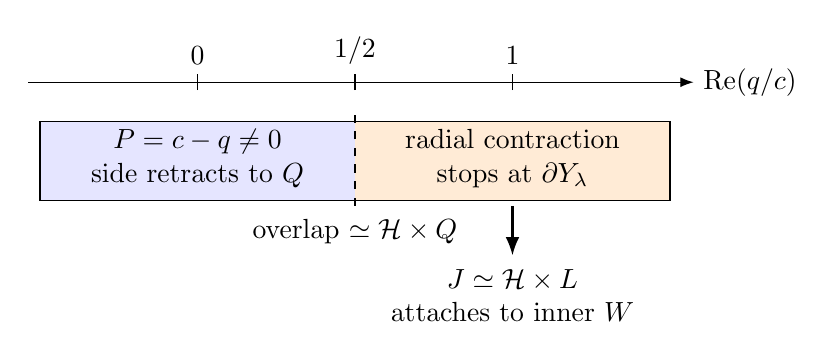
\begin{tikzpicture}[x=1cm,y=1cm,>=Latex]
  \draw[->] (-4.15,1.5)--(4.3,1.5)
    node[right] {\(\operatorname{Re}(q/c)\)};
  \foreach \x/\lab in {-2/0,0/{1/2},2/1}
    {\draw (\x,1.4)--(\x,1.6) node[above] {\(\lab\)};}
  \fill[blue!10] (-4,0) rectangle (0,1);
  \fill[orange!16] (0,0) rectangle (4,1);
  \draw (-4,0) rectangle (4,1);
  \draw[dashed,thick] (0,-.07)--(0,1.15);
  \node[align=center] at (-2,.53)
    {\(P=c-q\ne0\)\\ side retracts to \(Q\)};
  \node[align=center] at (2,.53)
    {radial contraction\\ stops at \(\partial Y_\lambda\)};
  \node[below] at (0,-.12) {overlap \(\simeq\Hh\times Q\)};
  \draw[->,thick] (2,-.07)--(2,-.7);
  \node[below,align=center] at (2,-.75)
    {\(J\simeq\Hh\times L\)\\ attaches to inner \(W\)};
\end{tikzpicture}

\caption{The exterior cut uses \(q=h\), with the full page equation
\(P=c-q\), shown by its real-part projection. The left side keeps
\(P\) away from zero; the right
side retracts to the actual interface \(J\) by stopping weighted
radial contraction at \(\partial Y_\lambda\), where \(P\) need not
vanish. The interface continuation identifies \(J\) with
\(\Hh\times L\). The overlap-to-\(J\) map is
\(\mathrm{id}_{\Hh}\times(Q\to L)\). This is schematic:
the disk radius \(\varepsilon\) and point \(c\) are not to scale.}
\label{fig:split}
\end{figure}

\begin{lemma}[Mayer--Vietoris boundary]\label{lem:mv}
The full page has an exact sequence
\begin{equation}
0\longrightarrow K\longrightarrow H_3(\T_s)
\xrightarrow{\partial} H\otimes E
\xrightarrow{\overline{1\otimes\tau}}H/\pi_*D.
\label{eq:tube-13}
\end{equation}
The image of the exterior page in \(H_3(\T_s)\) maps
isomorphically under \(\partial\) to \(H\otimes\ker\tau\).
\end{lemma}
\begin{proof}
Use Lemma~\ref{lem:continuations} to compute the exterior at \(s=0\).
Normalize \(c>0\), and put \(q=h\). Cut at
\(\operatorname{Re}q=c/2\), as in Figure~\ref{fig:split}, calling
the left and right pieces \(A\) and \(B\), respectively.
On \(A\), \(|P|=|c-q|\ge c/2\), so the removed inner block is
absent. The allowed \(P\)-values form a convex region avoiding zero,
and the boundary estimates of Lemma~\ref{lem:boundary} trivialize
its \(P\)-pages with their outer cuts. Contracting the base by the
positive weights of \(h\) and carrying these pages through the
trivialization retracts \(A\) to \(Q\).

On \(B\), choose one boundary-respecting trivialization of the
\(h\)-pages over the convex regular-value region
\(\{|q|\le\varepsilon,\ \operatorname{Re}q\ge c/2\}\).
It can agree near \(c\) with the page labels used in
Lemma~\ref{lem:continuations}. For \(v=(y,z,w)\), define the
radius of its block by
\[
 r(v)=\max\left\{
 (|y|/M)^{1/\alpha},\ (|z|/M)^{1/\beta},\ |w|
 \right\}.
\]
The exterior condition is \(\lambda\le r(v)\le\rho\).
Scale \(v\) by the cone weights, from \(t=1\) down to
\(t=\lambda/r(v)\), while retaining its \(h\)-page label and setting
\[
 v_t=(t^\alpha y,t^\beta z,tw),\qquad
 q_t=c-t^{d_P}P(v)=(1-t^{d_P})c+t^{d_P}q,
 \qquad d_P=1+a\alpha.
\]
This keeps \(\lambda\le r(v_t)\le\rho\), and \(q_t\) stays in
the same convex \(h\)-region. The base-ball cut is preserved by
the trivialization. The homotopy therefore stays in \(B\) and
stops at the actual interface \(J\), fixing \(J\) pointwise.
At its endpoint \(v_L\in L\), the value is
\(q=c-P(v_L)\), generally different from \(c\).
The \(s=0\) interface continuation of
Lemma~\ref{lem:continuations} retains \(v_L\) and the base label
while changing this value to \(c\). It identifies the retract
with \(\Hh\times L\).

The seam values form the contractible interval
\(I=\{q=c/2+iu:|q|\le\varepsilon\}\).
Trivializing both page factors along \(I\) identifies the overlap
\(C=A\cap B\) with \(\Hh\times Q\times I\).
After contracting \(I\), its map to \(J\simeq\Hh\times L\)
is homotopic to \(\mathrm{id}_{\Hh}\times(Q\to L)\), where
\(Q\to L\) is weighted radial projection.
Both \(\Hh,Q\) have homotopy dimension one, so overlap
\(H_3=0\), while overlap \(H_2=H\otimes E\).
Moreover \(H_2(J)=H\otimes\Z/k=H/kH\) and
\(H_3(J)=\Z\). The latter generator maps to zero in
\(H_3(W)=K\): it is the full inner fiber over a regular
base point, whose \(H_3\) vanishes in the collapse model.
We record the orientation of the remaining interface map.
For a full-page
3-cycle write its exterior chain as \(e=e_A+e_B\), with
the inner chain \(w\) satisfying
\(\partial w=b_J,\ \partial e=-b_J\).
Define \(t_C=-\partial e_A\in Z_2(C)\). Then
\begin{equation}
\partial e_B=t_C-b_J,\qquad
z:=[t_C]\in H_2(C)=H\otimes E.
\label{eq:mv-cut-chain}
\end{equation}
This fixes the sign of the Mayer--Vietoris coordinate.
Let \(r_t:C\to B\), \(0\le t\le1\), be the stopped radial
homotopy just constructed, reparametrized to end in \(J\).
Its endpoint is the actual interface, with the same \(h\)-page
label under the compatible parameter rectangle. For the
cycle \(t_C\), the interval-first prism chain
\(S=r_*([0,1]\times t_C)\) has
\(\partial S=r_{1*}t_C-t_C\). Consequently
\begin{equation}
\partial(e_B+S)=r_{1*}t_C-b_J,\qquad
[b_J]=r_{1*}[t_C]
     =(1\otimes\tau)z\quad\hbox{in }H_2(J)=H/kH.
\label{eq:mv-strip}
\end{equation}
Under the degree-two normalization fixed after
\eqref{eq:tube-12}, this is the positive sign of the last arrow
in \eqref{eq:tube-13}.
The Mayer--Vietoris sequence now gives \eqref{eq:tube-13}, with final
map the quotient of \(1\otimes\tau\). Before \(W\) is
attached, exterior \(H_3\) differs from its
\(H\otimes\ker\tau\) contribution by precisely the image
of \(H_3(J)\); that image dies after attachment. This
proves the last statement.
\end{proof}

\section{The mod-four Bockstein and the exact lattice}\label{sec:integral-lattice}

The signed cut determines whether an exterior coordinate extends,
but an integral extension may have a fractional \(K_{\Q}\)-coordinate.
We determine that coordinate from the torsion boundary in \(H_2(J)\).
Write
\(\beta_{\rm Bock}:H_3(J;\Z/k)\to H_2(J)\) for the coefficient Bockstein,
using the same notation on restricted interfaces below.
Our convention is
\[
 \beta_{\rm Bock}[\overline C]=[\partial C/k]
\]
when \(C\) is an integral lift of a mod-\(k\) cycle
\(\overline C\). Under \eqref{eq:tube-11},
the signed root boundary views
a class of \(H_3(W;\Z/k)\) in \(D/kD\).
Let \(i=i_W:J\hookrightarrow W\) be the inclusion. We also write
\(\pi^!\) for the induced map \(H/kH\to D/kD\);
it is well defined because \(\pi^!(kH)\subseteq kD\).

\begin{lemma}[Bockstein equals finite-map transfer]\label{lem:bock}
For \(b\in H/kH=H_2(J)\), and any
\(\eta\in H_3(J;\Z/k)\) with \(\beta_{\rm Bock}\eta=b\),
\begin{equation}
\Psi(i_*\eta)=\pi^!b\pmod{kD},
\label{eq:tube-14}
\end{equation}
with the orientation of \(\Psi\) fixed after \eqref{eq:tube-12}.
\end{lemma}
\begin{proof}
First note that the ambiguity in \(\eta\) is reduction of
an integral class in \(H_3(J)=\Z\), and this class dies
in \(H_3(W)\) by Lemma~\ref{lem:mv}; thus the left-hand
side is unambiguous. It suffices to test on loops in
\(\Hh\) avoiding the finite branch discriminant.
Take \(w_0=\lambda/2\), with every root in
\(|w|<\lambda/4\). On the \(\theta=0\), \(h=c\)
model of the interface lens fiber, for \(p\in\Hh_c\)
the \(y\)-angle loop
\[
\gamma_p
=\{w=w_0,\ y=M\lambda^\alpha e^{i\phi},\
z=R_s(p,w_0)/y\}
\]
is the positive generator of \(H_1(L)=\Z/k\).
Indeed, at \(s=0\) the quotient
\((U,V)\mapsto(U^k,V^k,UV)\) lifts one positive turn of the
\(y\)-angle to a path ending at the deck transform
\((U,V)\mapsto(\omega U,\omega^{-1}V)\), where
\(\omega=e^{2\pi i/k}\). This generates the deck group.
The anchored \(s\)-continuation preserves the same oriented loop.
Let \(\widetilde\gamma_p\) denote its image on the actual
\(f_s=c\) interface under the explicit lift in
Lemma~\ref{lem:continuations}. That lift preserves the
\(h\)-page label \(p\), \(w_0\), and the exact \(y\)-angle,
though physical \(p\) moves. We compute below in the
\(\theta=0\) model and transport all relative classes to
the actual \(J\) and \(W\) by this isotopy. In the model,
the exact sequence of the pair \((L,\gamma_p)\) reads
\[
0=H_2(L)\to H_2(L,\gamma_p)
\xrightarrow{\partial}H_1(\gamma_p)=\Z
\to H_1(L)=\Z/k.
\]
It supplies a unique relative class \(S_p\) with
\(\partial S_p=k\gamma_p\).

Let \(F_p\) be the inner \(yz=R_s(p,w)\) fiber above a
regular \(p\), and let \(r_1,\dots,r_k\) be the roots in
the \(w\)-disk \(\Delta\). Let
\(X_p=X(\Delta,\{r_1,\dots,r_k\})\) be its balanced collapse core,
and let \(\gamma_p^{\rm core}\) be the circle over \(w_0\) in that
core. The balancing retraction does not fix the outer circle
\(\gamma_p\) pointwise. It gives a map of pairs
\[
 r_p:(F_p,\gamma_p)\longrightarrow(X_p,\gamma_p^{\rm core})
\]
that is an absolute homotopy equivalence and restricts to the
orientation-preserving circle homeomorphism retaining the \(y\)-angle.
The long exact sequences of the two pairs therefore show that
\(r_p\) induces an isomorphism on relative homology.
The constant-angle section of \(X_p\) is a disk meeting
\(\gamma_p^{\rm core}\) in one point. Adjoining that disk to the
relative subspace does not change relative homology; quotienting
it and \(\gamma_p^{\rm core}\) gives the circle suspension of
\(\Delta/(\{r_1,\dots,r_k,w_0\})\). Hence there is a natural isomorphism
\begin{equation}
\begin{split}
 H_2(F_p,\gamma_p)
 &\cong H_1(\Delta,\{r_1,\dots,r_k,w_0\})\\
 &\cong\{(a_1,\dots,a_k,a_0)\in\Z^{k+1}:
             a_1+\cdots+a_k+a_0=0\}.
\end{split}
\label{eq:tube-15}
\end{equation}
Use \(r_p\) to identify the oriented boundary classes of
\(\gamma_p\) and \(\gamma_p^{\rm core}\) in this calculation.
The class of an arc from \(w_0\) to \(r_i\), swept by
the \(y\)-angle, has root coefficient \(+1\) and
\(\gamma_p\)-boundary \(+1\), fixing the convention.
The image of \(S_p\) has \(a_0=-k\).
To compute this one fiber class, let \(r_i(t)\), \(0\le t\le1\),
be any braid of distinct roots in \(|w|<\lambda/4\), starting at
the roots of \(R_s(p,\cdot)\) and returning to the same unordered
root set. Put
\(Q_t(w)=\prod_{i=1}^k(w-r_i(t))\), so \(Q_1=Q_0\), and consider
the compact fibers \(F_t=\{yz=Q_t(w)\}\cap Y_\lambda\), their
boundaries \(L_t\), and the circles \(\gamma_t\) defined by the
same \(w_0\) and \(y\)-angle formula as \(\gamma_p\), with
\(R_s(p,w_0)\) replaced by \(Q_t(w_0)\).
Choose a smooth disk velocity \(v_t(w)\), supported in
\(|w|<\lambda/4\), equal to \(\dot r_i(t)\) near each moving root.
Then
\[
 \ell_t(w)=\frac{\dot Q_t(w)+Q'_t(w)v_t(w)}{Q_t(w)}
\]
extends smoothly across the roots. Indeed, near \(r_i(t)\), writing
\(Q_t=(w-r_i)B_{i,t}\) gives
\(\ell_t=(\dot B_{i,t}+\dot r_i B'_{i,t})/B_{i,t}\), with
\(B_{i,t}\ne0\).

The \(y\)- and \(z\)-faces of these fibers never meet, since
\(|Q_t(w)|\le(5\lambda/4)^4<M^2\lambda^4\).
Choose a smooth real cutoff \(\chi\), depending on
\(|y|^2,|z|^2\), that is zero near the \(y\)-face and one near the
\(z\)-face. The time-dependent lift
\[
 \dot w=v_t(w),\qquad
 \dot y=\chi\operatorname{Re}(\ell_t)y,\qquad
 \dot z=\bigl(\ell_t-\chi\operatorname{Re}(\ell_t)\bigr)z
\]
is smooth also at the roots and axes, and differentiation gives
\(\frac{d}{dt}(yz-Q_t(w))=\ell_t(yz-Q_t(w))\).
It is tangent to the \(y\)-face because \(\dot y=0\) there, to the
\(z\)-face because the coefficient of \(z\) is purely imaginary
there, and to the \(w\)-face because \(v_t=0\) there; these statements
also cover all corners. Compactness therefore gives transport of
the full triples \((F_t,L_t,\gamma_t)\). On \(\gamma_t\), it fixes
\(w_0\) and \(y=M\lambda^\alpha e^{i\phi}\) exactly, and gives
\(\dot z=\dot Q_t(w_0)/y\). Thus the return fixes the parametrized
circle \(\gamma_p\) pointwise.

The return maps of \((L,\gamma_p)\) and \((F_p,\gamma_p)\) commute
with inclusion. The former fixes the unique class \(S_p\) with
boundary \(k\gamma_p\); hence the latter fixes its image in
\(H_2(F_p,\gamma_p)\). To compute that same return map in
\eqref{eq:tube-15}, observe that the lift covers the disk flow
\(\psi_t\) of \(v_t\) and preserves the \(y\)-angle wherever defined.
It therefore intertwines the balancing collapses with the map
\((w,e^{i\phi})\mapsto(\psi_t(w),e^{i\phi})\) on the circle models;
collapsed root fibers are carried to collapsed root fibers.
The endpoint isomorphism in
\eqref{eq:tube-15} consequently sends its action to the permutation
of the root coefficients \(a_i\), with \(a_0\) fixed. Every root
permutation is available, and no additional term can occur because
the endpoint map is an isomorphism. Invariance of the image of
\(S_p\), together with \(a_0=-k\), now gives
\(a_1=\cdots=a_k=1\). Reducing \(S_p\) modulo \(k\)
closes its boundary and yields the diagonal root vector in the
absolute mod-\(k\) collapse homology.

Now work over an oriented base loop \(a\subset\Hh_c\) missing
branch values, still in the \(\theta=0\), \(h=c\) model. Write
\(\D_a=\pi^{-1}(a)\). Let \(W_a\) be the restriction of the inner
family \(F_p\) to \(p\in a\), and let \(J_a\subset W_a\) be its
restricted lens-interface family, with inclusion
\(i_a:J_a\hookrightarrow W_a\). The compatible isotopy of
Lemma~\ref{lem:continuations} transports their inclusions to the actual
pieces \(J\subset W\); the vertical maps below use this transport.
The same circle-first suspension and negative relative root boundary
define
\[
\Psi_a:H_3(W_a;\Z/k)\longrightarrow H_1(\D_a;\Z/k).
\]
The target remains the root homology in the \(h\)-model, with its
inclusion into \(H_1(\D;\Z/k)\). The actual covering monodromy
over \(a\) may be a smaller braid subgroup, with several orbits.
Over a small arc
\(I\subset a\), the same transport tracks roots and preserves the
circle angle. Collapse relative to the constant-angle
section, take the relative root boundary, and slice
over \((I,\partial I)\). Each operation is natural
under this product trivialization: on chains its
relative map is the fiber operation times
\([I,\partial I]\). Restriction and inclusion give
the following naturality diagram:
\begin{equation}
\begin{array}{ccccc}
H_3(J_a;\Z/k)&\xrightarrow{i_{a*}}&H_3(W_a;\Z/k)
 &\xrightarrow{\Psi_a}&H_1(\D_a;\Z/k)\\
\downarrow&&\downarrow&&\downarrow\\
H_3(J;\Z/k)&\xrightarrow{i_*}&H_3(W;\Z/k)
 &\xrightarrow{\Psi}&H_1(\D;\Z/k).
\end{array}
\label{eq:tube-16}
\end{equation}
The common orientation of the normal circle fixes the
sign of the two right-hand maps. The fiber endpoint
calculation gives the diagonal root vector after
slicing the top row at \(p\).
We construct a Bockstein lift on \(J_a\) by first closing a swept
chain at the seam. The anchored circles trace the base-first torus
\(a\times\gamma_p\) over \(a\). Cut \(a\) at one point, choose a
representative
\(S_0\) of \(S_p\) with \(\partial S_0=k\gamma_p\), transport it
along the resulting interval, and call its endpoint \(S_1\).
The anchored circle is fixed at the seam, so
\(\partial S_0=\partial S_1=k\gamma_p\). Uniqueness of the relative
class makes \(S_1-S_0\) a null-homologous \(2\)-cycle in \(L\);
choose a seam cap \(C_a\) with
\(\partial C_a=S_1-S_0\), using \(H_2(L)=0\).
Let \(T_a\) be the interval-first sweep. Then
\[
 \partial T_a=S_1-S_0-k(a\times\gamma_p),\qquad
 \partial(T_a-C_a)=-k(a\times\gamma_p).
\]
The second boundary is divisible by \(k\), so the reduction is a cycle.
Set
\[
\eta_a=-[(T_a-C_a)\bmod k]\in H_3(J_a;\Z/k),
\]
and let \(\eta\) be its image in \(H_3(J;\Z/k)\) under inclusion
and transport.
The Bockstein convention gives
\(\beta_{\rm Bock}\eta_a=[a\times\gamma_p]\) on \(J_a\), and
\(\beta_{\rm Bock}\eta=[a\times\gamma_p]\) on \(J\), with the
torus transported in the second identity. Changing the cap changes
\(\eta_a\) by the reduction modulo \(k\) of an integral class from
\(H_3(L)\), and changes \(\eta\) by its image. The integral class
maps to zero in \(H_3(W)\) by the fiber
calculation used in Lemma~\ref{lem:mv}, so its mod-\(k\) image
dies as well.
Thus both
\(\Psi i_*\eta\) and the full transfer \(\pi^![a]\) are
images of classes in \(H_1(\D_a;\Z/k)\).
Choose the slice away from the seam. Slicing at \(p\in a\) sends each oriented component circle
of the unramified cover \(\D_a\to a\) to the sum of the
roots in its monodromy orbit. Distinct orbits have
disjoint supports, so this slice map is injective on
\(H_1(\D_a;\Z/k)\). The fiber calculation gives the
diagonal root vector for \(\Psi_a i_{a*}\eta_a\), and the
full transfer has the same vector. Their classes agree
already in \(H_1(\D_a;\Z/k)\), hence in \(D/kD\).
Such base loops generate
\(H_1(\Hh)\), proving \eqref{eq:tube-14}.
\end{proof}

We now define the rational coordinates of an integral page class.
For \(x\in H_3(\T_s)\), let \(z=\partial x\) and
\(b=(1\otimes\tau)z\in H/kH\). Since
\(kz\in H\otimes\ker\tau\), Lemma~\ref{lem:mv} supplies a unique
\(x_{\rm ext}(kz)\) in the exterior image with coordinate \(kz\).
Define
\[
u:=kx-x_{\rm ext}(kz)\in K,\qquad
x\longmapsto (u/k,z)\in K_\Q\oplus(H\otimes E)_\Q.
\]
We call \(u\) the integral numerator of the inner coordinate.
The Bockstein lemma supplies \(+\pi^!b\); the cap calculation below
shows that subtracting the interface cap gives the numerator residue
\(u\equiv-\pi^!b\pmod{kD}\).

\begin{lemma}[integral extension]\label{lem:lattice}
In these rational coordinates, the image of \(H_3(\T_s)\) is exactly
the lattice
\[
\Lambda_\pi=
\left\{(\pr l,z): l\in D,\ z\in H\otimes E,\quad
\pi_*l\bmod kH=(1\otimes\tau)z\right\}
\subset K_\Q\oplus(H\otimes E)_\Q
\]
from \eqref{eq:tube-1}, where
\(\pr l=l-k^{-1}\pi^!\pi_*l\).
\end{lemma}
\begin{proof}
Fix \(x\), with \(z,b,u\) as above. Orient \(J\) as the outgoing
boundary of \(W\), and represent \(x\)
by page chains \(w\in C_3(W)\) and
\(v\in C_3(M_{\rm ext})\) with
\(\partial w=b_J\) and \(\partial v=-b_J\).
The oriented prism calculation \eqref{eq:mv-cut-chain}--\eqref{eq:mv-strip}
gives \([b_J]=b=(1\otimes\tau)z\) in
\(H_2(J)=H/kH\). Because this
group is killed by \(k\), choose an
integral \(A\in C_3(J)\) with
\(\partial A=k b_J\). Write
\(i_{\rm ext}:J\hookrightarrow M_{\rm ext}\) for the exterior inclusion.
The chains
\begin{equation}
 w_k:=kw-i_{W*}A,\qquad
 v_k:=kv+i_{{\rm ext}*}A
\label{eq:tube-16a}
\end{equation}
are closed in their respective pieces.
Their sum in the full page is \(kx\):
the two copies of \(A\) cancel on \(J\).
The exterior class \([v_k]\) has
second coordinate \(kz\), hence is
\(x_{\rm ext}(kz)\) in the full page;
its possible \(H_3(J)\) ambiguity dies
after attaching \(W\). Consequently
\(u=[w_k]\in K\). Modulo \(k\),
\([w_k]=-i_{W*}[A\bmod k]\).
The coefficient convention gives
\(\beta_{\rm Bock}[A\bmod k]=[\partial A/k]=[b_J]=b\).
With the \(\Psi\) orientation fixed after
\eqref{eq:tube-12}, Lemma~\ref{lem:bock}
gives \(\Psi i_*[A\bmod k]=+\pi^!b\).
The preceding minus sign in
\([w_k]=-i_{W*}[A\bmod k]\) therefore gives
\begin{equation}
 u\equiv-\pi^!b\pmod{kD}.
\label{eq:tube-17}
\end{equation}
Choose \(b_H\in H\) lifting \(b\) and put
\(l=(u+\pi^!b_H)/k\). The congruence makes
\(l\in D\), and
\(\pi_*l=b_H\), \(\pr l=u/k\).
Conversely, if \(l,z\) obey the condition in
\eqref{eq:tube-1}, the last arrow of \eqref{eq:tube-13} kills \(z\).
Choose any \(x\) with that \(z\), and put
\[
u_x:=kx-x_{\rm ext}(kz)\in K,\qquad
u_l:=kl-\pi^!\pi_*l\in K.
\]
Here \(u_x\) is the integral numerator of the rational inner
coordinate \(u_x/k\).
By \eqref{eq:tube-17}, \(u_x-u_l\in K\cap kD\).
This intersection equals \(kK\):
if \(kv\in K\) for \(v\in D\), then
\(k\pi_*v=0\), and \(H\) is torsion free,
so \(v\in K\). Adjust \(x\) by
\((u_l-u_x)/k\in K\) through the first
arrow of \eqref{eq:tube-13}. The adjusted class has
rational coordinate \((\pr l,z)\).
Thus every pair in \eqref{eq:tube-1} occurs.
Replacing \(b_H\) by
\(b_H+kh\) changes \(l\) by \(\pi^!h\) and
does not change \(\pr l\), so the coordinate
description is independent of the lift.
\end{proof}

We have now located every integral page class in
\(K_{\Q}\oplus(H\otimes E)_{\Q}\). The residue condition in
\eqref{eq:tube-1} retains the particular projection \(\pi_*\);
an abstract isometry of the two plane Seifert lattices does not
identify it. It remains to compute the ordered filling form on
this exact lattice.

\section{The two filling summands}\label{sec:filling-summands}

The integral lattice is now fixed by \eqref{eq:tube-1}. We compute
its ordered filling form on the two rational summands, first by
separating inner and exterior fillings and then by examining the
normal disks of an inner filling. Throughout, the first filling
bounds the first cycle on the reference page, and the second bounds
the positive neighboring-page transport of the second cycle. The boundary continuations
preserve these complex page values and arise from oriented ambient
isotopies, so they preserve this order and the intersection numbers.

\begin{lemma}[orthogonality and exterior form]\label{lem:exterior}
The \(K_\Q\) and \((H\otimes E)_\Q\) summands are
orthogonal for the tube filling form. The
second summand has form \(s_h\otimes e\).
\end{lemma}
\begin{proof}
The inner classes bound in the acyclic
\(\widehat W\). For an exterior page class
representing an element of \(H\otimes\ker\tau\),
its image in \(H_3(\widehat M_{\rm ext})\)
may be nonzero. The compatible sublevel continuations take \(\widehat J\) to
the product of the acyclic base total of \(h\) with \(L\).
Its integral \(H_3\) is therefore generated by one oriented lens
fiber. Lemma~\ref{lem:acyclic} then gives
\(H_3(\widehat J)\cong H_3(\widehat M_{\rm ext})\cong\Z\). Under the interface continuation, the
inclusion \(J\hookrightarrow\widehat J\) sends the oriented
lens-fiber generator of \(H_3(J)\) to a generator of
\(H_3(\widehat J)\). Subtract the
corresponding integral multiple of the
page-interface generator, which is zero
in the full page. The adjusted exterior
class bounds in \(\widehat M_{\rm ext}\).
This can be done compatibly under a short
value-circle transport arc. Put the two
fillings on opposite sides of a bicollar
of \(\widehat J\); their interiors are then
disjoint, proving orthogonality.

Continue the exterior piece to \(s=0\).
Its full lift to \((U,V)\) lies off the
cone vertex, where the cyclic map is an
orientation-preserving unramified \(k\)-cover.
Thus intersections of full lifts are \(k\)
times intersections downstairs. This covering count uses the
original fillings off the cone vertex. In the contractible
upstairs total, the filling pairing is unchanged when those
fillings are replaced by the radial fillings used below.
The smooth join calculation follows Sakamoto's product formula
\cite[Theorem~2, p.~715]{Sakamoto1974} and the product construction of
\cite{KauffmanNeumann1977}; the cone extension
and integral gluing were established here. The lifted cycles
also live in the full smooth tube
for \(h+\widetilde P\), whose total is
contractible by weights. Its page
Mayer--Vietoris coordinate is
\(H\otimes H_1(\widetilde Q)\);
the lift of \(z\in H\otimes E\) has
coordinate \((1\otimes\tr)z\).
For pure tensors, represent this class
by the join of loops in the two factor
pages, varying their values as
\((tc,(1-t)c)\), \(0\le t\le1\).
It meets the equal-value cut in the
product of the two loops. Fill the join
by the two factor radial cone fillings
with values in
\(\{(t,t')c:t,t'\ge0,\ t+t'\le1\}\).
The two ordered fillings meet only at
the common origins of the factors
because their neighboring rays are
disjoint away from zero. Near each
intersection they are products of
two real 2-dimensional filling
intersections. Their Koszul sign is
\((-1)^{2\cdot2}=+1\); any uniform
join-orientation sign occurs in both
fillings and cancels. Hence the upstairs
form is \(s_h\otimes\widetilde s\).
Division by \(k\) gives \(s_h\otimes e\)
downstairs. Since \(kE\subseteq\ker\tau\), exterior classes span their
rational summand, so the identity holds
on all of it.
\end{proof}

The exterior calculation has now fixed both cross terms and the
product form. The remaining calculation compares an inner filling
with the plane filling that supplies its class in \(K\).

\begin{lemma}[the inner negative sign]\label{lem:inner}
The restriction of the filling form to
\(K\) is \(-s_d|_K\).
\end{lemma}
\begin{proof}
Starting from two plane fillings, we build relative chains and sweep
them by the normal circle at two distinct balancing radii.
The sweeps will be separated away from the root
locus, so each remaining intersection is an intersection of the
plane fillings multiplied by the sign of two normal disks.
We first construct the sweeps as filling chains and then compute
that normal sign.

Use the \(h\)-model of Lemma~\ref{lem:continuations} over the value disk
\(\{|v|\le\delta\}\). For \(|v|\le\delta\), set
\[
G_v=(\mathcal B\cap\{h=v\})\times\{|w|\le\lambda\},\qquad
\widehat G=(\mathcal B\cap\{|h|\le\delta\})\times\{|w|\le\lambda\},
\]
and let \(\widehat\D=\widehat G\cap\{R_s=0\}\) be its root total.
By the selected plane cut calculation used in
Lemma~\ref{lem:acyclic}, \(\widehat\D\) is acyclic; the same holds
for \(\widehat G\), the base total times a disk.

Choose the initial chains as finite integral sums of mapped oriented
simplices, piecewise smooth after compatible subdivision. The swept
chains will be continuous at the conical strata described below and
piecewise smooth elsewhere. Intersections mean transverse intersections of
the maps on their smooth common contacts, counted with their integer
coefficients; we retain set notation for their images.
For two classes \(l_1,l_2\in K\), take \(c_1\) as the reference
page and \(c_2\) as its positive neighbor, and represent \(l_i\)
by cycles on the root page in \(G_{c_i}\). Their images vanish in
\(H_1(G_{c_i})\) because \(l_i\in K=\ker\pi_*\).
This vanishing and the acyclicity of \(\widehat\D\) let us choose
surface chains \(\Sigma_i\subset\widehat\D\) with
\(\partial\Sigma_i=l_i\) and \(V_i\subset G_{c_i}\) with
\(\partial V_i=-l_i\). Arrange \(\Sigma_1,\Sigma_2\)
transversely in the real four-dimensional \(\widehat\D\),
with generic \(V_i\) and disjoint page-boundary collars.
Since \(H_2(\widehat G)=0\),
the closed chain \(\Sigma_i+V_i\) bounds a
\(3\)-chain \(\Gamma_i\subset\widehat G\).
Prescribe a collar of the \(\Sigma_i\)-face on which
\(R_s=t\ge0\) is a positive-real normal coordinate.
Near \(l_i\), make its normal lift tangent to \(h=c_i\),
possible because \((h,R_s)\) is a submersion there, and join
it to a collar of \(V_i\). Keep these collars fixed.
Perturb only the remaining interiors of \(\Gamma_1,\Gamma_2\)
relative to their boundary chains, and make
\[
I_i=(\Gamma_i\setminus\text{prescribed collar})\cap\widehat\D
\]
transverse there. Each \(I_i\) is a real one-dimensional
chain, with any endpoints on the prescribed \(V_i\) contacts.
Relative transversality gives
\(I_1\cap\Sigma_2=\Sigma_1\cap I_2=I_1\cap I_2=\varnothing\):
the respective dimension sums are \(1+2<4\) and \(1+1<4\).
Separate their finite boundary contacts in the distinct
page-value collars. Thus the only common root contacts are
the prescribed \(\Sigma_1\cap\Sigma_2\) intersections.

Choose distinct \(\sigma_1,\sigma_2\) sufficiently near
\(\lambda^{(\alpha-\beta)/2}\) that the strict balancing bounds
in Lemma~\ref{lem:acyclic} hold for both; their circles then stay
inside \(Y_\lambda\).
Sweep each \(\Gamma_i\) by the \(y\)-angle
using \(|y|=\sigma_i\sqrt{|R_s|}\),
\(|z|=\sigma_i^{-1}\sqrt{|R_s|}\), and \(z=R_s/y\)
away from the root.
This is the chain-level relative suspension
\(C_3(\widehat G,\widehat\D)\to C_4(\widehat W)\).
To realize it by mapped chains, triangulate the domains compatibly
with the prescribed collars, the transverse root curves, and their
boundary faces. Sweep each oriented top simplex, collapse its
circle over the root, and push the resulting top chain into
\(\widehat W\). The internal faces cancel with the original
chain coefficients. The \(\Sigma_i\)-face is zero in the relative
complex, so it contributes no boundary after collapse.
Write \(\mathfrak S\) also for the circle-first suspension of
Section~\ref{sec:circle-collapse} followed by this collapse and
pushforward. Give the sweep the negative of the raw product
orientation. In the relative quotient chain complex the two
relevant signs are
\[
 \partial\bigl(-\mathfrak S(\Gamma_i)\bigr)
    =+\mathfrak S(V_i),\qquad
 -\partial_{\D}V_i=l_i.
\]
The second identity says that this boundary is the positive
\(K\)-page class in the convention fixed after \eqref{eq:tube-12}.
The same reversal for both fillings does not change their
intersection product.

We now verify that the mapped sweeps have the claimed filling
boundary at root contacts.
Along the prescribed normal collar,
the collapsed circle is the center of a disk. At an incidental
transverse root curve \(I_i\), the local quotient is
\(I_i\times\operatorname{cone}(T^2)\): its torus link is closed
and oriented. The oriented top simplices of a triangulated cone
have cancelling internal faces, and its tip is not a
codimension-one face; hence this local model contributes no
additional chain boundary.
The map extends continuously to \(y=z=0\) there.

We next locate the intersections of the two sweeps.
Where \(R_s\ne0\), the sweeps are
disjoint at a common base point because their \(|y|\) differ.
Where \(R_s=0\), their possible common contacts are
\((\Sigma_1\cup I_1)\cap(\Sigma_2\cup I_2)
=\Sigma_1\cap\Sigma_2\). Thus all intersections occur
above the prescribed transverse surface intersections.
In particular, the conical tips over \(I_i\) are disjoint from
the other swept chain. A small general-position approximation in
disjoint neighborhoods of those tips, fixed on the prescribed
collars and with each boundary kept in its assigned page, preserves
the filling classes and adds no intersections. Thus the filling
intersection is computed entirely on the smooth prescribed collars.
Only the intersection sign of the normal disks remains.
In complex normal coordinates \(y,z\)
there, each swept collar is the real
disk \(z=\sigma_i^{-2}\overline y\).
In real coordinates \(y=x+it\), its
graph map has matrix
\(\mathrm{diag}(\sigma_i^{-2},
-\sigma_i^{-2})\), so the ordered
intersection determinant is
\[
\det\bigl(
\mathrm{diag}(\sigma_2^{-2},-\sigma_2^{-2})
-\mathrm{diag}(\sigma_1^{-2},-\sigma_1^{-2})
\bigr)
=-(\sigma_2^{-2}-\sigma_1^{-2})^2<0.
\]
Both collar disks have the same orientation relative to
the complex \(y\)-orientation (both are reversed by the
chosen sweep), so their common reversals cancel in the
intersection product. Also,
interchanging a disk past a root
surface contributes
\((-1)^{2\cdot2}=+1\).
Thus every root-surface
intersection sign is reversed.
The root-surface filling
intersections are exactly
\(s_d(l_1,l_2)\) by the common
nearby-page convention, proving
the lemma. Changing the
uniform sign of the \(K\)-coordinate
does not change this bilinear
restriction.
\end{proof}

\noindent\emph{Proof of Theorem~\ref{thm:tube}.}
Lemmas~\ref{lem:boundary}, \ref{lem:continuations}, and
\ref{lem:isolation} provide a
proper Milnor-model tube with
a unique critical point. The acyclicity
proved in Lemma~\ref{lem:acyclic} completes
the comparison in Lemma~\ref{lem:local},
identifying its page and pairing with the
ordinary local Milnor data.
Lemmas~\ref{lem:acyclic},
\ref{lem:mv}, \ref{lem:bock},
and \ref{lem:lattice} give the
integral lattice \eqref{eq:tube-1}, while
Lemmas~\ref{lem:exterior} and
\ref{lem:inner} give \eqref{eq:tube-2}.
\qed

\section{From the integral lattice to an embedded link}\label{sec:fourfold-arithmetic}

We now compare the two actual Milnor lattices supplied by
Theorem~\ref{thm:tube}. Two boundary classes of the cone page give
rational Seifert isometries that are integral at complementary sets
of primes. We compare these two maps and use strong approximation to
replace their local choices by one integral isometry. The final
subsection then identifies the embedded links. Throughout, we use the
full integral lattice formula, including its mod-four boundary
condition and the signs of both filling forms.

The parameters \(r,n_0,n_1,a,b,\alpha,\beta\) remain the single
choice fixed in Lemma~\ref{lem:simultaneous-parameters}. Its analytic
bounds are already available. We begin with the remaining
divisibility facts and positive indices needed for the real-sign
calculation.

\begin{lemma}[Divisibility and positive indices]\label{lem:parameter-indices}
For the parameters fixed in Lemma~\ref{lem:simultaneous-parameters}, put
\[
 g=\gcd(a,b),\qquad m=4ab+a+b.
\]
Then \(a,b\equiv2\pmod5\), \(5\nmid g\), and
\(g\ge 2^{r-1}>5\). For each \(q\in\{1,4\}\), there are positive
integers \(i,j\) satisfying
\[
 i\equiv j\pmod4,\qquad \frac{bi+aj}{m}=\frac q5 .
\]
\end{lemma}

\begin{proof}
Both \(n_0,n_1\) are \(2\pmod5\), so
\((n_j^2-1)/4\equiv2\pmod5\). Thus \(a,b\equiv2\pmod5\)
and \(5\nmid g\). Also \(2^r\mid n_j-1\) and \(2\mid n_j+1\),
whence \(2^{r-1}\mid a,b\) and \(g\ge2^{r-1}>5\).

Write \(a=ga'\), \(b=gb'\), with \(\gcd(a',b')=1\).
The desired index equations, on writing \(i=j+4t\), become
\[
 (a'+b')j+4b't=\frac{qm}{5g}.
\]
Reduction modulo five gives \(m=4ab+a+b\equiv0\pmod5\);
since \(5\nmid g\), we have \(5\mid m/g\). Let
\(d=\gcd(a'+b',4b')\). The equality \(\gcd(a'+b',b')=1\)
gives \(d\mid4\), and \(d\) also divides
\(m/g=4ga'b'+a'+b'\). Hence \(d\mid m/(5g)\), so the
displayed equation has integer solutions for \(q=1,4\).
Its homogeneous solutions change \(j\) by \(4b'/d\); choose a
solution with \(1\le j\le4b'/d\le4b'\). For \(q=1\),
\[
 \frac{m}{5g}
   =\frac{4ga'b'+a'+b'}5
   >4a'b'
\]
because \(g>5\). Thus
\(i=(qm/(5g)-a'j)/b'>0\) for both values of \(q\).
\end{proof}

Put $k=4$.  For $\nu\in\{0,1\}$ let
$\pi_\nu\colon\mathcal D_\nu\to\mathcal H$ be the degree-$k$ map of
plane-curve Milnor pages constructed above.  Write
\[
 \begin{aligned}
 H&=H_1(\mathcal H;\mathbb Z),&
 D_\nu&=H_1(\mathcal D_\nu;\mathbb Z),\\
 K_\nu&=\ker(\pi_{\nu*}\colon D_\nu\to H),&
 \operatorname{pr}_\nu l
   &=l-\frac1k\pi_\nu^!\pi_{\nu*}l.
 \end{aligned}
\]
The transfer identities are $\pi_{\nu*}\pi_\nu^!=k$ and
$s_{d_\nu}(\pi_\nu^!x,l)=s_h(x,\pi_{\nu*}l)$ in both argument orders.
In particular $\operatorname{pr}_\nu$ projects rationally onto $K_\nu$
along $\pi_\nu^!H_{\mathbb Q}$, orthogonally for the Seifert forms.
The plane-curve argument has supplied an integral Seifert isometry
\begin{equation}\label{eq:arith-plane-isometry}
 \mathcal I\colon(D_0,s_{d_0})\xrightarrow{\ \sim\ }(D_1,s_{d_1}),
\end{equation}
and has shown that their monodromies are semisimple at eigenvalue
$1$ and at primitive fifth roots.  These facts are separate inputs to the
present section.

Let $Q$ be a Milnor page of $P=w(y^a+z^b)$ on the cone
$S=\{yz=w^4\}$, let $E=H_1(Q;\mathbb Z)$, and let
$\tau\colon E\to H_1(\operatorname{link}(S))=\mathbb Z/4$ be induced by
weighted radial projection $Q\to\operatorname{link}(S)$, equivalently
by page inclusion in the link open-book model. The rational form $e$
on $E$ is one fourth of the upstairs Seifert pairing of transferred
cycles. Theorem~\ref{thm:tube} identifies the Milnor lattice and its
Seifert form $s_\nu$, in one convention on both sides, as follows:
\begin{equation}\label{eq:arith-input-lattice}
 \begin{split}
 F_\nu&=(K_\nu)_{\mathbb Q}\oplus(H\otimes E)_{\mathbb Q},\\
 s_\nu&=(-s_{d_\nu}|_{K_\nu})\perp(s_h\otimes e),\\
 \Lambda_\nu&=
 \left\{(\operatorname{pr}_\nu l,z):
       l\in D_\nu,\ z\in H\otimes E,\quad
       \pi_{\nu*}l\equiv(1\otimes\tau)z\pmod{4H}\right\}.
 \end{split}
\end{equation}
The rational vector space $F_\nu$ is $\Lambda_\nu\otimes\mathbb Q$.
Every later localization uses this complete integral lattice with the
displayed residue condition; all tensor products and pairings use the
displayed identification.

\subsection{Two boundary vectors}\label{subsec:arith-boundary}
The graph index \(\nu\in\{0,1\}\) and the boundary index
\(j\in\{0,1\}\) are independent.

The quotient map $(U,V)\mapsto(U^4,V^4,UV)$ identifies $S$ with
$\mathbb C^2/\mu_4$, with action $(U,V)\mapsto(\omega U,\omega^{-1}V)$.
Upstairs the cone-page equation is
\begin{equation}\label{eq:arith-upstairs-page}
 \widetilde P(U,V)=UV(U^{4a}+V^{4b}).
\end{equation}
Orient the boundary class $b_0\in E$ of the $y$-axis as a complex
branch and the class $b_1$ of the $z$-axis oppositely to its complex
orientation.  The quotient lens space has $H_1=\mathbb Z/4$; with the
positive $y$-axis class as generator, both have $\tau(b_j)=1$.

\begin{lemma}[Boundary pairings]\label{lem:arith-boundary}
The classes $b_0,b_1$ are fixed by the page monodromy, and
\begin{equation}\label{eq:arith-boundary-pairings}
 \begin{aligned}
 e(b_j,b_j)&=-\frac{n_j^2}{4},&
 e(b_0,b_1)&=-\frac14,\\
 4e(b_j,x)&\equiv-\tau(x)\pmod4&&(x\in E).
 \end{aligned}
\end{equation}
\end{lemma}

\begin{proof}
The weighted rotation preserves each axis, hence its boundary homology
class.  Transfer of either axis boundary is a single boundary circle of
the upstairs plane-curve page.  In a positive plane-curve Seifert
convention, the pairing of two distinct complex branch boundaries is their
positive local intersection multiplicity.  The sum of all oriented
boundary classes is zero, so the self-pairing of the $V=0$ boundary is
$-(1+4a)=-n_0^2$, and that of $U=0$ is $-(1+4b)=-n_1^2$.
The two axes meet once.  Reversing the second orientation gives the
mixed value $-1$ upstairs.  Division by the covering degree proves the
first two formulas.

The integer-valued functional $x\mapsto4e(b_j,x)$ reduces modulo $4$
through $\tau$.  Indeed a loop whose $\tau$-class is zero lifts closed;
its full transfer consists of four deck translates, and the transferred
axis class is deck invariant.  The four Seifert pairings are equal, so
their sum is divisible by $4$.  A class in $\ker\tau$ can be represented
by such loop systems, and $\tau(b_j)=1$ generates $\mathbb Z/4$.
Evaluation at $b_j$ gives $4e(b_j,b_j)=-n_j^2\equiv-1\pmod4$,
proving the last congruence.
\end{proof}

\subsection{Two complementary local splittings}\label{subsec:arith-local}

We first make explicit why the Seifert operator of $e$ is defined.
Over $\mathbb Q$, transfer identifies $E_{\mathbb Q}$ with the
deck-invariant summand of the upstairs page homology. Let
$\widetilde s$ be the nondegenerate upstairs Milnor Seifert form
in the same ordered convention.
The deck transformations are $\widetilde s$-isometries, so their
averaging projection $p=\frac14\sum_{\gamma\in\mu_4}\gamma$ satisfies
$\widetilde s(px,y)=\widetilde s(x,py)$. Its image and kernel are
therefore orthogonal in both orders, and the restriction of
$\widetilde s$ to the invariant summand is nondegenerate. Under
transfer, $e$ is one fourth of this restriction,
so $e$ is nondegenerate and
$A_e=e^{-1}e^{\mathsf t}$ is the restriction of
$\widetilde A=\widetilde s^{-1}\widetilde s^{\mathsf t}$.
The weighted rotation $\widetilde M$ has rational weights $b/m,a/m$,
hence finite order, and commutes with the deck action. The identity
relating a plane-curve Seifert form and monodromy reads
$\widetilde A=\widetilde M^\varepsilon$ for one fixed
$\varepsilon\in\{1,-1\}$ in the common convention. The same
$\varepsilon$ applies to the base page. Thus $A_e$
has finite order and fixes the classes $b_j$, since the weighted
rotation fixes their transferred axis boundaries.

Set $v_j=b_j/n_j\in E_{\mathbb Q}$.  Since $A_eb_j=b_j$,
the form $e$ pairs $v_j$ symmetrically with every vector:
$e(v_j,x)=e(x,A_ev_j)=e(x,v_j)$.
Equation \eqref{eq:arith-boundary-pairings} gives
\begin{equation}\label{eq:arith-v-norm}
 e(v_j,v_j)=-\frac14.
\end{equation}
For a rational prime $\ell\nmid n_j$, write
$E_{\mathbb Z_\ell}=E\otimes\mathbb Z_\ell$ and let
\[
 \tau_{\mathbb Z_\ell}\colon E_{\mathbb Z_\ell}
 \longrightarrow(\mathbb Z/4)\otimes\mathbb Z_\ell
 \cong\mathbb Z_\ell/4\mathbb Z_\ell
\]
be the scalar extension of $\tau$. For $x\in E_{\mathbb Z_\ell}$,
the value $-4e(v_j,x)$ lies in $\mathbb Z_\ell$, since
$4e(b_j,x)$ is integral and $n_j$ is a unit. In this coefficient
ring, \eqref{eq:arith-boundary-pairings} gives
\[
 -4e(v_j,x)\equiv\tau_{\mathbb Z_\ell}(x)
       \pmod{4\mathbb Z_\ell}.
\]
The target is zero at odd primes. At $\ell=2$, the congruence uses
$n_j\equiv1\pmod4$ from Lemma~\ref{lem:simultaneous-parameters}.

\begin{lemma}[Local splitting]\label{lem:arith-local-splitting}
For every rational prime $\ell\nmid n_j$, the lattice
$E_{\mathbb Z_\ell}$ has the following $\mathbb Z_\ell$-module
splitting, orthogonal for the $\mathbb Q_\ell$-valued form $e$:
\[
 E_{\mathbb Z_\ell}=
 \mathbb Z_\ell v_j\perp U_{j,\ell},
 \qquad U_{j,\ell}\subset\ker(\tau_{\mathbb Z_\ell}).
\]
For $\nu=0,1$ this induces an integral Seifert isometry
\begin{equation}\label{eq:arith-local-alpha}
 \begin{split}
 \alpha_{\nu,j}\colon
 &(D_\nu,-s_{d_\nu})_{\mathbb Z_\ell}
       \perp(H\otimes U_{j,\ell},s_h\otimes e)
       \xrightarrow{\ \sim\ }(\Lambda_\nu,s_\nu)_{\mathbb Z_\ell},\\
 &(l,u)\longmapsto
 \bigl(\operatorname{pr}_\nu l,\ \pi_{\nu*}l\otimes v_j+u\bigr).
 \end{split}
\end{equation}
It also holds over $\mathbb Q$.
\end{lemma}

\begin{proof}
The coefficient of $x\in E_{\mathbb Z_\ell}$ on $v_j$ is
$c_j(x)=-4e(v_j,x)$.  It is integral because $4e(b_j,x)$ is integral and
$n_j$ is a unit in $\mathbb Z_\ell$, and it sends $v_j$ to $1$ by
\eqref{eq:arith-v-norm}.  Its kernel $U_{j,\ell}$ is therefore an
integral orthogonal summand. The local congruence above gives
$\tau_{\mathbb Z_\ell}(U_{j,\ell})=0$. At $\ell=2$,
$c_j(x)\equiv\tau_{\mathbb Z_2}(x)\pmod{4\mathbb Z_2}$
because $n_j\equiv1\pmod4$;
at odd primes the target of $\tau_{\mathbb Z_\ell}$ is zero.
Thus the projection $x\mapsto c_j(x)v_j$ is integral also at
$\ell=2$: all divisions are by the unit $n_j$.

The image of \eqref{eq:arith-local-alpha} satisfies the lattice
congruence \eqref{eq:arith-input-lattice}.  Conversely, write the second
coordinate of an arbitrary lattice element as
$z=x_H\otimes v_j+u$.  Its congruence says
$x_H-\pi_{\nu*}l\in4H_{\mathbb Z_\ell}$.  Replacing $l$ by
\[
 l+\pi_\nu^!\left((x_H-\pi_{\nu*}l)/4\right)
\]
is legitimate even at $\ell=2$, because the numerator belongs to
$4H_{\mathbb Z_\ell}$. It does not alter $\operatorname{pr}_\nu l$ and makes its image under
$\pi_{\nu*}$ equal to $x_H$.  This proves surjectivity; injectivity
follows from the rational direct sum.

The $H\otimes U_{j,\ell}$ summand is orthogonal to the image of $D_\nu$.
On two vectors from $D_\nu$, transfer adjunction gives
\[
 s_{d_\nu}(\operatorname{pr}_\nu l,
                  \operatorname{pr}_\nu l')
 =s_{d_\nu}(l,l')-
        \frac14s_h(\pi_{\nu*}l,\pi_{\nu*}l').
\]
The product-form contribution on $v_j$ is the negative of the last
fraction, by $e(v_j,v_j)=-1/4$.  Combined with the leading minus sign
on $K_\nu$ in \eqref{eq:arith-input-lattice}, the result is
$-s_{d_\nu}(l,l')$, as claimed.
\end{proof}

Use the fixed plane isometry $\mathcal I$ from
\eqref{eq:arith-plane-isometry} on the $D$-summands and the identity
on $H\otimes U_{j,\mathbb Q}$.  The rational versions of
\eqref{eq:arith-local-alpha} give Seifert isometries
\begin{equation}\label{eq:arith-two-J}
 J_j=\alpha_{1,j}(\mathcal I\oplus1)\alpha_{0,j}^{-1}
 \colon(F_0,s_0)\xrightarrow{\ \sim\ }(F_1,s_1).
\end{equation}
They are lattice isometries at every $\ell\nmid n_j$.  No compatibility
between $\mathcal I$ and the two maps $\pi_\nu$ is required: those maps enter
only through the explicit changes of coordinates $\alpha_{\nu,j}$.
Since $\gcd(n_0,n_1)=1$, the two isometries $J_0,J_1$
cover all primes locally.

\subsection{The discrepancy on two primary sectors}
\label{subsec:arith-correction}

The local choices will give one integral isometry if their discrepancy
\[
 \Delta=J_0^{-1}J_1\colon F_0\longrightarrow F_0
\]
can be corrected at the primes dividing $n_0$ without disturbing the
source lattice at the other primes. We first identify the rational
isometry groups containing this discrepancy. The normalized boundary
vectors $v_0,v_1$ are exchanged by a reflection; comparison of the corresponding
reflections on $F_0$ and $F_1$ will remove the determinant and spinor
obstructions. To state that comparison, we describe the two monodromy
sectors on which the reflections act.

Let $A_\nu=s_\nu^{-1}s_\nu^{\mathsf t}$ be the Seifert operator.
It is an isometry of $s_\nu$.  By the rational orthogonal decomposition
\eqref{eq:arith-input-lattice}, its action is the operator of $d_\nu$
on $K_\nu$ and the tensor product of the operators of $h$ and $e$
on $H\otimes E$.  The operator of $e$ has finite order because
\eqref{eq:arith-upstairs-page} is weighted homogeneous; the operator
of $h$ has order $5$.  The plane-curve semisimplicity input therefore
shows that $A_\nu$ is semisimple at $1$ and at primitive fifth roots.
Let
\[
 F_{\nu,1}=\ker(A_\nu-1),\qquad
 F_{\nu,5}=\ker\Phi_5(A_\nu),\qquad
 B_\nu=s_\nu+s_\nu^{\mathsf t}.
\]
These primary spaces split off rationally and orthogonally, because
their eigenvalue sets are stable under inversion.  On them $B_\nu$
is nondegenerate: $s_\nu^{\mathsf t}=s_\nu A_\nu$, hence
$B_\nu=s_\nu(1+A_\nu)$, and neither primary sector has eigenvalue
$-1$.  On $F_{\nu,1}$ it is a rational quadratic form.  On
$F_{\nu,5}$ the action of $A_\nu$ makes the space a vector space over
$L=\mathbb Q(\zeta)$, $\zeta=e^{2\pi i/5}$, with
$L^+=\mathbb Q(\zeta+\zeta^{-1})$. Define the $L$-valued form
$\mathfrak h_{\nu,5}$ on $F_{\nu,5}$ by trace duality:
\[
 \operatorname{Tr}_{L/\mathbb Q}\!\left(c\,\mathfrak h_{\nu,5}(x,y)\right)
   =B_\nu(cx,y)\qquad(c\in L).
\]
The $B_\nu$-adjoint of $c$ is $\bar c$, because $A_\nu$ is a
$B_\nu$-isometry. Nondegeneracy of the field trace pairing therefore
gives sesquilinearity and Hermitian symmetry for $L/L^+$, and
nondegeneracy follows from that of $B_\nu$. The same identity shows
that every $L$-linear $B_\nu$-isometry preserves $\mathfrak h_{\nu,5}$.

For the base form on $H_{\mathbb Q}$, set
\[
 A_h=s_h^{-1}s_h^{\mathsf t},\qquad
 H^{(1)}=\ker(A_h-1),\qquad H^{(5)}=\ker\Phi_5(A_h).
\]
With the same convention as above, $A_h=M_h^\varepsilon$.

\begin{lemma}[The discrepancy lifts]\label{lem:arith-discrepancy}
The rational Seifert isometry
$\Delta=J_0^{-1}J_1$ acts as the identity outside
$F_{0,1}\oplus F_{0,5}$.  Its restriction to $F_{0,1}$ lifts to the
rational points of the spin group of $B_0|F_{0,1}$.  Its restriction to
$F_{0,5}$ lies in the special unitary group of the $L/L^+$ Hermitian
form.
\end{lemma}

\begin{proof}
The two $v_j$ have the same norm $-1/4$, while
$e(v_0,v_1)=-1/(4n_0n_1)$.  Therefore
\[
 w=v_0-v_1,\qquad
 e(w,w)=-\frac12\left(1-\frac1{n_0n_1}\right)\ne0.
\]
The vector $w$ is monodromy fixed and hence pairs symmetrically
for $e$.  Reflection
\[
 R_w(x)=x-\frac{2e(x,w)}{e(w,w)}w
\]
is consequently an $e$-isometry commuting with monodromy, and it
exchanges $v_0,v_1$.  Define $\rho_\nu$ on $F_\nu$ as identity on
$(K_\nu)_{\mathbb Q}$ and $1_H\otimes R_w$ on
$(H\otimes E)_{\mathbb Q}$.  This is a rational Seifert
involution.  Let $\mathcal R_\nu$ be identity on $D_\nu$ and
$1_H\otimes R_w$ from $H\otimes U_{0,\mathbb Q}$ to
$H\otimes U_{1,\mathbb Q}$.  Equation
\eqref{eq:arith-local-alpha} gives
$\rho_\nu\alpha_{\nu,0}=\alpha_{\nu,1}\mathcal R_\nu$.
The same $R_w$ occurs for both coverings, so the square formed by
$\mathcal R_0,\mathcal R_1$ and $\mathcal I\oplus1$ commutes.  Consequently
\begin{equation}\label{eq:arith-J-conjugacy}
 J_1=\rho_1J_0\rho_0^{-1},\qquad
 \Delta=(J_0^{-1}\rho_1J_0)\rho_0^{-1}.
\end{equation}
The minus space of $\rho_\nu$ is
$W_\nu=H_{\mathbb Q}\otimes\mathbb Qw$. Its restricted Seifert form
is $e(w,w)s_h$, so its Seifert operator is $A_h$. In particular it
lies entirely in $F_{\nu,1}\oplus F_{\nu,5}$. Both factors of
\eqref{eq:arith-J-conjugacy}, and therefore $\Delta$, act
identically on every other rational primary summand.

The minus spaces within the two primary sectors are
\[
 W_{\nu,1}=H^{(1)}\otimes\mathbb Qw,\qquad
 W_{\nu,5}=H^{(5)}\otimes\mathbb Qw.
\]
The canonical map $x\otimes w\mapsto x\otimes w$ from $W_0$ to
$W_1$ preserves the restricted Seifert and symmetric forms and
intertwines $A_h$. It therefore restricts to isometries on the
individual sectors displayed above. These restrictions are
nondegenerate: $e(w,w)\ne0$, and $s_h+s_h^{\mathsf t}$ is
nondegenerate on both $H^{(1)}$ and $H^{(5)}$. Since the Seifert
isometry $J_0$ intertwines $A_0$ and $A_1$, composition with
$J_0^{-1}$ identifies, separately on each sector, the minus spaces
of $\rho_0$ and $J_0^{-1}\rho_1J_0$.
On $F_{0,5}$ the isometry $\Delta$ commutes with the $L$-action
and preserves the Hermitian form recovered from $B_0$.  The two
involutions in \eqref{eq:arith-J-conjugacy} have the same
$L$-dimension of their minus spaces, so their $L$-determinants
cancel: $\det_L\Delta=1$.
It is therefore an $L^+$-rational special-unitary element.

On $F_{0,1}$ the same comparison gives determinant $1$.  The
spinor norm of an involution with nondegenerate minus space is the
product, modulo rational squares, of the quadratic values of an
orthogonal basis of that space.  The minus spaces just identified
are isometric, so their spinor norms are
equal and cancel in the product.  Thus $\Delta$ has trivial
spinor norm.  The standard exact sequence for
$\operatorname{Spin}\to\operatorname{SO}$ now supplies a rational
spin lift
\cite[Section~C.5, paragraph before Example~C.5.5 and Lemma~C.5.8]{Conrad2014Reductive}.
\end{proof}

\subsection{Noncompact real factors}\label{subsec:arith-real}

Lemma~\ref{lem:arith-discrepancy} places the required correction in a
spin group over $\mathbb Q$ and a special unitary group over $L^+$.
Strong approximation in these groups requires noncompactness at an
archimedean place. We now prove the corresponding indefiniteness of
the quadratic and Hermitian forms. Both signs come from holomorphic
and antiholomorphic classes of the cone page.

\begin{lemma}[Real signs]\label{lem:arith-real-signs}
The quadratic form $B_\nu|F_{\nu,1}$ is indefinite and has dimension at
least five.  The Hermitian form on $F_{\nu,5}$ has dimension at least two
over $L$ and is indefinite at the real place of $L^+$ indexed by
the pair $\{\zeta,\bar\zeta\}$. Both assertions hold for $\nu=0,1$.
\end{lemma}

\begin{proof}
By Lemma~\ref{lem:plane-data}, the rational primary parts
$H^{(1)}$ and $H^{(5)}$ have dimensions two and four, respectively,
and together equal
$H_{\mathbb Q}$. Their eigenvalue sets are stable under inversion, so
they are nondegenerate orthogonal summands for $s_h$. The restriction
to $H^{(1)}$ is symmetric, and each complex primitive fifth
eigenspace is one-dimensional and pairs nondegenerately with its
inverse eigenspace.

To obtain both Hodge signs in the primitive fifth eigenspaces of
$E_{\mathbb C}$, we construct holomorphic forms with inverse primitive
fifth characters. Their conjugate antiholomorphic classes will give
opposite cup-product signs. Set $m=4ab+a+b$, and write
$a=ga'$, $b=gb'$ with $\gcd(a',b')=1$.  The weights of $U,V$ in
\eqref{eq:arith-upstairs-page} are $b/m,a/m$.  For $q=1$ and $q=4$
there are positive integers $i,j$, congruent modulo $4$, with
\begin{equation}\label{eq:arith-weight-indices}
 \frac{bi+aj}{m}=\frac q5.
\end{equation}
The existence and positivity of these two index pairs were proved in
Lemma~\ref{lem:parameter-indices}.

On the smooth affine curve $\widetilde P=1$, the differential
\begin{equation}\label{eq:arith-eigenform}
 \omega_{i,j}=U^{i-1}V^{j-1}
        \frac{dU}{\partial_V\widetilde P}
       =-U^{i-1}V^{j-1}
        \frac{dV}{\partial_U\widetilde P}
\end{equation}
is regular and nonzero.  The second expression is used where
$\partial_V\widetilde P=0$.  Its deck character is
$\omega^{i-j}=1$, so it descends to the quotient, and its weighted
rotation character is $e^{2\pi iq/5}$.
To obtain the needed holomorphic classes, we check that these
differentials extend across every end of the normalized
compactification. At an end put
$u=\operatorname{ord}U$, $v=\operatorname{ord}V$.
If $4au<4bv$, then $u<0$ and $v=-(4a+1)u$; the order of
\eqref{eq:arith-eigenform} is
$(i-(4a+1)j)u-1\ge0$.  Here
$i<4a+1$, because \eqref{eq:arith-weight-indices}, $q\le4$ and
$j\ge1$ give $bi\le4m/5-a<b(4a+1)$.
The case $4bv<4au$ is symmetric, using the second expression and
$j<4b+1$.  In the remaining case $4au=4bv<0$, leading terms in
$U^{4a}+V^{4b}$ cancel and
$\operatorname{ord}(\partial_V\widetilde P)=u+4bv$.
There is a positive integer $c$ with $(u,v)=-c(b',a')$; the order is
\[
 (i-1)u+(j-1-4b)v-1
 =c\left(1-\frac q5\right)\frac mg-1\ge0.
\]
These are all possible ends, since one of $U,V$ has a pole.

The two differentials for $q=1,4$ thus give nonzero holomorphic
forms on the smooth compactification with characters $\zeta$ and
$\bar\zeta$.  Complex conjugation gives antiholomorphic forms of
the opposite characters.  The cup-product Hermitian form has
opposite signs on holomorphic and antiholomorphic forms. Poincar\'e
duality exchanges reciprocal characters and gives opposite signs for the
Hermitian intersection form on the corresponding homology classes. Since both characters
have been constructed, each of the two homology eigenspaces has both
signs. With complex coefficients, the map from affine-page homology to
compactification homology is surjective and preserves intersections. Average a linear section
of this map over the finite group generated by the commuting deck
transformations and weighted rotation. The resulting equivariant
section lifts the classes with their characters and intersection
numbers unchanged. Transfer over $\mathbb C$ identifies
the deck-invariant part with $E_{\mathbb C}$ and preserves the
monodromy characters.  Since $e-e^{\mathsf t}$ is, up to our common
Seifert convention, the page intersection form, the Hermitian form
$i(e-e^{\mathsf t})(x,\bar x)$ has both signs in each of
$E_\zeta$ and $E_{\bar\zeta}$.

We transfer these signs to the fixed quadratic sector by tensoring
a primitive base eigenspace with the inverse eigenspace of $E$.
After complexifying, choose $\lambda\in\{\zeta,\bar\zeta\}$ and a
nonzero $x\in\ker(A_h-\lambda)\subset H_{\mathbb C}$. This eigenspace is one-dimensional and
pairs nondegenerately with its inverse eigenspace. The preceding
statement that both signs occur applies to
$\ker(A_e-\lambda^{-1})\subset E_{\mathbb C}$
under either inverse monodromy convention. For $y$ in this eigenspace, put
\[
 I_H=i(s_h-s_h^{\mathsf t})(x,\bar x),\qquad
 I_E=i(e-e^{\mathsf t})(y,\bar y).
\]
These are real, and $I_H\ne0$. The relation $s^{\mathsf t}=sA$ in
each factor, together with the vanishing of $s_h(x,x)$ and $e(y,y)$
when $\lambda^2\ne1$, gives
\[
 B_\nu(x\otimes y+\bar x\otimes\bar y,\,
       x\otimes y+\bar x\otimes\bar y)
 =-\frac{4I_HI_E}{|1-\lambda|^2}.
\]
The vectors in this display lie in $F_{\nu,1}\otimes_{\mathbb Q}\mathbb R$, and the two
signs of $I_E$ prove that $B_\nu|F_{\nu,1}$ is indefinite. These
tensors and their conjugates already contribute at least four real dimensions.
The invariant part of $H$ has dimension two, and $b_0$ is a nonzero
invariant vector of $E$ by \eqref{eq:arith-boundary-pairings}; its
tensor contributes at least two more dimensions.

For the Hermitian sector, we tensor the primitive eigenspace of $E$
with a fixed base vector. Choose $x\in H\cap H^{(1)}$ with $s_h(x,x)\ne0$.
Such an integral vector exists: the nondegenerate symmetric
restriction to $H^{(1)}$ has a rational vector of nonzero norm, and
clearing denominators puts it in $H$. Tensor $x$ with $E_\zeta$.
This lies in the
$\zeta$ component of $F_{\nu,5}$ for one of the two inverse
monodromy conventions.  If the eigenvalue of $A_e$ on $E_\zeta$
is $\lambda\in\{\zeta,\zeta^{-1}\}$, then on this eigenspace
\[
 (e+e^{\mathsf t})(y,\bar y)
 =\frac{1+\lambda^{-1}}{i(1-\lambda^{-1})}
       i(e-e^{\mathsf t})(y,\bar y),
\]
and the displayed ratio is a nonzero real number.  The two signs
found above therefore give both signs for the Hermitian form of
$B_\nu$ at this real embedding.  Its dimension is at least two.
\end{proof}

\subsection{A single integral isometry}\label{subsec:arith-approximation}

We can now combine the rational lift of the discrepancy with the real
noncompactness just proved. The approximation will be imposed inside
stabilizers of the full lattice $\Lambda_0$, so it preserves the
mod-four gluing even though the rational primary decomposition need
not split that lattice integrally.

\begin{proposition}[Integral Seifert congruence]
\label{prop:arith-integral-congruence}
For the two germs constructed above, the two integral Milnor Seifert
forms $(\Lambda_0,s_0)$ and $(\Lambda_1,s_1)$ are isometric.
\end{proposition}

\begin{proof}
By Lemma~\ref{lem:arith-real-signs},
$G_1=\operatorname{Spin}(F_{0,1},B_0)$ is a connected, simply
connected, absolutely almost simple group over $\mathbb Q$ of
quadratic dimension at least five
\cite[Proposition~C.3.10, Lemma~C.4.1, Proposition~C.4.10, and Example~C.6.6]{Conrad2014Reductive}.
The proved indefiniteness makes it noncompact over $\mathbb R$.
The second correction group
$G_5=\operatorname{SU}(F_{0,5},\mathfrak h_{0,5})$
is connected, simply connected,
and absolutely almost simple over $L^+$: after algebraic closure it
is $\operatorname{SL}_d$, with $d\ge2$
\cite[Proposition~24.40(b), equation~(158), and Summary~21.96]{Milne2022}.
It is noncompact at the real place found in
Lemma~\ref{lem:arith-real-signs}.
We use
$G=G_1\times\operatorname{Res}_{L^+/\mathbb Q}G_5$,
acting on the indicated primary spaces and as identity on their
$s_0$-orthogonal primary complement. The Spin action preserves
$B_0$ and commutes with $A_0=1$ on $F_{0,1}$. The special-unitary
action preserves the Hermitian form, hence $B_0$, and commutes with
$A_0$ on $F_{0,5}$ by $L$-linearity. On both sectors $1+A_0$ is
invertible and
\[
 s_0=B_0(1+A_0)^{-1}.
\]
Consequently this action of $G$ preserves the Seifert form $s_0$.
We obtain the density assertion for $G$ by treating its two factors
separately.

The strong-approximation theorem of Kneser and Platonov, in the
precise form of \cite[Theorem~2.3]{Rapinchuk2014}, says that for a
connected, simply connected, absolutely almost simple group over a
number field, noncompactness at a place in the omitted finite set
implies density of rational points in the adeles away from that set.
Apply it to $G_1$ over $\mathbb Q$ and to $G_5$ over $L^+$, omitting
all archimedean places.  Restriction of scalars and a finite
product give density of $G(\mathbb Q)$ in $G(\mathbb A_f)$.

Write $\rho\colon G\to\operatorname{GL}(F_0)$ for this rational
action.  Lemma~\ref{lem:arith-discrepancy} gives a rational lift
$\widetilde\Delta\in G(\mathbb Q)$ with
$\rho(\widetilde\Delta)=\Delta$.  For each rational prime $\ell$,
put $a_\ell=\widetilde\Delta$ if $\ell\mid n_0$, and
$a_\ell=1$ otherwise. The tuple $\mathbf a=(a_\ell)_\ell$ has finite
support and lies in $G(\mathbb A_f)$. We seek one rational point
$g_{\mathrm{rat}}\in G(\mathbb Q)$ whose localizations
$g_{\mathrm{rat},\ell}$ differ from these selected corrections by
automorphisms of the full source lattice:
\[
 \rho(a_\ell^{-1}g_{\mathrm{rat},\ell})
       (\Lambda_0\otimes\mathbb Z_\ell)
   =\Lambda_0\otimes\mathbb Z_\ell
       \quad\text{for every }\ell.
\]
To construct a suitable open neighborhood of $\mathbf a$, define the
exact source-lattice stabilizer
\[
 C_\ell=\left\{\gamma\in G(\mathbb Q_\ell):
   \rho(\gamma)(\Lambda_0\otimes\mathbb Z_\ell)
          =\Lambda_0\otimes\mathbb Z_\ell\right\}.
\]
Each $C_\ell$ is compact open.  Here the spin action has finite
central kernel, so it need not be faithful; compactness follows
from finiteness of the covering onto its algebraic image.
For the adelic topology we only need compact opens inside these
stabilizers.  Spread out $G$ and its rational action on $F_0$ to a
smooth affine group scheme $\mathcal G$ over $\mathbb Z[1/N]$,
enlarging $N$ so that the action preserves
$\Lambda_0\otimes\mathbb Z[1/N]$.  At every $\ell\nmid N$ its
standard compact open $\mathcal G(\mathbb Z_\ell)$ lies in $C_\ell$.
For each of the finitely many primes $\ell\mid N$, choose a compact
open subgroup $K_\ell\subset C_\ell$; at the other primes put
$K_\ell=\mathcal G(\mathbb Z_\ell)$.  Then
$\mathcal K=\prod_\ell K_\ell$ is compact open in $G(\mathbb A_f)$ and
$\mathbf a\mathcal K$ is an open coset contained in the desired set of local
integral corrections.

At $\ell\nmid n_0$, Lemma~\ref{lem:arith-local-splitting}
makes $J_0$ an integral lattice isometry.  At $\ell\mid n_0$
we have $\ell\nmid n_1$, so $J_0\rho(a_\ell)=J_1$ is integral.
Consequently
\[
 J_0\rho(a_\ell)(\Lambda_0\otimes\mathbb Z_\ell)
                  =\Lambda_1\otimes\mathbb Z_\ell
       \quad\text{for every }\ell.
\]
Density supplies $g_{\mathrm{rat}}\in G(\mathbb Q)\cap\mathbf a\mathcal K$.
Writing $g_{\mathrm{rat},\ell}=a_\ell k_\ell$
with $k_\ell\in K_\ell\subset C_\ell$
shows that
$J_0\rho(g_{\mathrm{rat}})$ induces the same local lattice equality at every prime.
A full $\mathbb Z$-lattice in a rational vector space is the
intersection of its localizations at all primes; applying this to
both sides yields
$J_0\rho(g_{\mathrm{rat}})\Lambda_0=\Lambda_1$.
Since $J_0$ and $\rho(g_{\mathrm{rat}})$ preserve their respective Seifert forms,
this is the asserted integral congruence.
\end{proof}

\subsection{The embedded links}\label{subsec:arith-links}

The final step uses Kato's Theorem~B and his definition in Section~2
\cite[pp.~454--455]{Kato1974}. The theorem
has no homotopy-sphere hypothesis on the binding. In his terminology,
a spinnable structure
on an oriented $(2n+1)$-manifold is an open book with compact
$2n$-dimensional page $F$, characteristic diffeomorphism fixed
near $\partial F$, and an identification of its open-book quotient
with the ambient manifold.  It is simple when $F$ is obtained from
a ball by handles of index at most $n$.  Theorem~B states that for
$n\ge3$ two such structures on $S^{2n+1}$ with congruent integral
Seifert matrices are isomorphic.  Kato explicitly notes on p.~454
that this applies to isolated complex hypersurface singularities;
his footnote credits Durfee's independent result
\cite{Durfee1974}.

For each function constructed above, the origin is an isolated
critical point in a smooth complex four-dimensional chart.  Its
Milnor open book lies on the standard $S^7$, so $n=3$; its compact
page has real dimension six and its binding has real dimension five.
We use the analytic form of Milnor's theorem, recalled explicitly by
N\'emethi \cite[pp.~63--64]{Nemethi1999SeifertInfinity}: an isolated
analytic germ supplies a simple spinnable Milnor structure. In our
four-dimensional charts this gives the handle bound required by Kato.

We also specify the characteristic diffeomorphism near the binding.
The Milnor open book has the local product model
$\partial F\times D^2$, with the fibration given by the angular
coordinate on $D^2\setminus\{0\}$. Choose the horizontal angular
field to be the product rotation on a smaller such neighborhood,
and extend it over the complement by a partition of unity among
horizontal lifts. Its return after one turn fixes a collar of
$\partial F$ pointwise.

Theorem~\ref{thm:tube} identifies \eqref{eq:arith-input-lattice}
with the actual integral Milnor Seifert forms in the same ordered
push-off convention. Proposition~\ref{prop:arith-integral-congruence}
is an onto isometry of these integral lattices. In integral bases
of the page groups $H_3(F;\mathbb Z)$, its matrix is therefore
unimodular and gives exactly an integral congruence of Seifert
matrices. The common complex and positive-target orientations
make any universal sign or transpose in the conversion to Kato's
convention the same on both sides, so the congruence is preserved.
Kato's Theorem~B now gives an orientation-preserving diffeomorphism
$\phi$ of the two sphere-link pairs: the isomorphism of open books
carries pages and therefore their embedded boundaries.

To pass to the germs, use the analytic ambient-pair cone theorem,
attributed to \L{}ojasiewicz in
\cite[Theorem~1.4]{Massey2015LeCycles}. It identifies each sufficiently
small ball pair, including its center, with the cone on its
sphere-link pair. The map
$[u,t]\mapsto[\phi(u),t]$ is a homeomorphism of the two cone pairs.
Conjugating it by the two analytic pair-cone homeomorphisms gives
the required homeomorphism germ of ambient pairs.

\begin{proof}[Proof of Theorem~\ref{thm:main}]
Proposition~\ref{prop:ambient-orders} and Lemma~\ref{lem:isolation}
give smooth ambient fourfold germs and reduced isolated functions of
orders five and four. Theorem~\ref{thm:tube} identifies their actual
integral Milnor Seifert forms, and Proposition~\ref{prop:arith-integral-congruence}
gives an integral congruence. The Kato argument above identifies their
embedded links. The analytic pair-cone construction above extends that equivalence
to an ambient homeomorphism germ, proving the assertion.
\end{proof}

\bibliographystyle{plain}
\bibliography{references}
\end{document}
